\documentclass[conference]{IEEEtran}
\usepackage[english]{babel}

\usepackage{float} 
\usepackage{url}  
\usepackage{multirow}
\usepackage{caption}
\usepackage{subcaption}
\usepackage{booktabs}
\usepackage{cite}
\pagestyle{plain}
\usepackage{amsmath}
\usepackage{float}
\usepackage{tikz}
\usetikzlibrary{shapes.geometric, arrows, positioning}
\usepackage{placeins}
\usepackage{comment}
\usepackage{tabularx}
\ifCLASSINFOpdf
  \usepackage[pdftex]{graphicx}
\fi

\hyphenation{op-tical net-works semi-conduc-tor}

\begin{document}


\title{Sentiment Classification of Financial Texts Using the Financial Phrasebank Dataset}

\author{\IEEEauthorblockN{\\ Hugo Veríssimo}
\IEEEauthorblockA{Complements of Machine Learning 24/25\\
University of Aveiro\\
Aveiro, Portugal\\
hugoverissimo@ua.pt}
\and
\IEEEauthorblockN{\\ João Cardoso}
\IEEEauthorblockA{Complements of Machine Learning 24/25\\
University of Aveiro\\
Aveiro, Portugal\\
joaopcardoso@ua.pt}}

\maketitle
\thispagestyle{plain}

\begin{abstract}
This work explores financial sentiment analysis using the Financial PhraseBank dataset, a benchmark in the field for its annotated financial news snippets. The performance of three different models, fastText, LSTM, and BERT, is evaluated and compared on a selected subset with 75\% annotator agreement. BERT-based models significantly outperform the others, motivating further refinement through data augmentation and a novel weighted training strategy that incorporates annotator agreement levels during training. The proposed models achieve performance in line with, or surpassing, literature baselines, demonstrating the importance of both architecture selection and annotation-informed weighting schemes in financial NLP.
\end{abstract}

\begin{quote}
\small
\noindent
\textbf{Keywords:}  financial sentiment analysis, Financial PhraseBank, deep learning, natural language processing
\end{quote}

\IEEEpeerreviewmaketitle


\section{Introduction}

With the ever-increasing volume of information created and distributed by the minute, access to fast and reliable analysis of encountered information is more important than ever. Especially with the democratized access to financial instruments and capital markets, where individuals have the possibility to invest in virtually any company on the stock exchange, it is important to have ways to leverage against giant institutions with hundreds of financial analysts at their disposal. 

Historically, financial analysis relied heavily on fundamental analysis (examining earnings, balance sheets, annual financial reports), which required extensive knowledge in the field (also the strategy that made Warren Buffett one of the richest men in the world), along with technical analysis (studying price and volume trends). Around 2010, after the 2008 global financial crisis, there was a surge in news analysis to evaluate the tone and derive investment strategies from it \cite{tetlock2007giving}. Due to the lack of domain specific lexicon these analysis were falible, until the work by Loughran and McDonald was published, a financial lexicon based on 10-K forms (i.e., annual financial reports) and dictionaries \cite{loughran2011liability}. This allowed to use more sofisticated analysis rather than using the presence of negative words as a signal to sell.

Upon the launch of Twitter, information streams increased dramatically, making more and more data available for analysis. But, machine learning was not heavily used, as most data was not annotated, or there was very little data with high-quality annotations. In 2014, P. Malo \textit{et al.} published a fundamental dataset for financial sentimental analysis, that is still used, the Financial Phrasebank. It is unique, for the inclusion of important aspects as directional expressions (e.g., profits decreased), entity polarity shifts (e.g. profits may be negative if decreased), and phrase level context \cite{malo2014good}.

With this, machine learning models started finding their place, as the field of natural language processing (NLP) grew and niche fields such as financial investments found more useful data. This work explores the Financial Phrasebank dataset by implementing different machine learning and deep learning models to evaluate the sentiment of sentences related to financial news.

\section{State of The Art}

The field of NLP has grown drastically in the past decade, progressing from recurrent neural networks (RNN) and related models such as Long-Short Term Memory (LSTM), to the transformers-type models, large language models (LLM) and text generative models as ChatGPT. With the Financial Phrasebank the field expanded into financial analysis, with several works of relevance being published in recent years.

In the work of Araci (2019), the author developed a BERT-based model trained specifically on texts with financial data. BERT, Bidireccional Encoder Representations from Transformers, is a large language model developed by Google (2018), benefitting largely from the fact that it can "hold" in memory large chunks and in both directions, simultaneously \cite{devlin2019bert}. The fact that it is built on the Transformer encoder architecture, it can weigh the importance of different words in a sentence by using a self-attention. The model is pre-trained  on large unlabelled corpora (e.g., Wikipedia, BookCorpus), and can be fine-tuned for specific purposes. In this work, the end model was trained on  domain specific corpus such as TRC2-financial data and financial specific texts (over ~440 000 sentences), and then fine tuned with the Financial Phrasebank. The model achieved an accuracy of 97\% and a F1-score of 95\% on the Financial Phrasebank dataset with 100\% agreement, but only 86\% and 84\%, respectively, on the dataset with all levels of agreement (the agreement will be further detailed in the Methodology section) \cite{araci2019finbert}. 

Later on the model was further improved by Sun \textit{et al.} (2025), EnhancedFinSentiBERT, by including dictionary embeddings, expanded corpus that deversified the pre-training stage drastically, and a novel neutral sentiment module, that further enhanced the distinction between neutral and weak sentiments, resulting F1-score (87\%). The pre-training stage benefited from the large diversity of the corpus, going from a few million tokens to 2.4 B tokens with the latest version \cite{sun2025financial}.

In a similar direction, but at the fine-tuning level, Atsiwo (2024) improved the data used in fine-tuning, considering that most datasets have relatively short sentences ($<$ 100 tokens), failing to leverage the full context window  of LLMs like BERT (512 tokens). This was achieved by augmenting  the training data with synthetic sentences generated by GPT-4, with accuracy of 89\% and F1-score of 88\% for 50\% agreement dataset \cite{atsiwo2024financial}. 

GPT has been used with different purposes, as in the work by Fatouros \textit{et al.} (2023), where GPT-3.5Turbo was used for zero-shot sentiment classification. These conditions are harder on the model, as it never undergoes specific training for the context, relying solely on its pre-training (hence the poorer performance against finely tuned models). Under the same conditions (not using the Financial PhraseBank, but scraped headlines related with forex trading), it outperformed finely-tuned models with an accuracy of 75\% and F1-score of 74\% (finely tuned models in zero-shot conditions achieve accuracy of 56\% and F1-score of 55\%) \cite{fatouros2023chatgpt}.

The BERT model was revisited by different researchers, but a new iteration from Facebook AI was proposed (2019) named RoBERTa (Robustly Optimized BERT Approach) was developed, that used a signficantly larger corpus for training (10x larger), and a dynamic masking technique during training, that allowed the model to learn new contextual relations while using the same sentences, making it more robust \cite{liu2019roberta}. This model was used to develop financial models, where the work Choe \textit{et al.} (2023) is worth mentioning, where a large corpus of financial texts were fed to the model for training, from a range of sources (e.g., Reuters, SEC fillings, EIA). The model (FiLM, Financial Language Model) benefited from the diversity of training data, rather than simply focusing on fine tuning with highly curated data, showing improved generalization and better metrics than FinBERT and RoBERTa (accuracy 86\%, F1-score 84\%) \cite{choe2023exploring}.

These models are improving substantially over the years, but it is different to put them to test against a controlled dataset from using them in real life, and the variety included as consequence. Competitions such as FinNLP help drive research in this field, by posing ever more diversified test sets, aiming to improve the robustness of models, and the solutions developed by the researchers.


\section{Methodology}

To address the problem of sentiment classification in sentences related to financial investment, a pipeline was set up for training and testing using the Financial PhraseBank for three types of models, where the best was further explored and tuned for different tests. The dataset and setup are detailed in the following subsections.

\subsection{Dataset}

The Financial PhraseBank is a widely used benchmark dataset for financial sentiment analysis. It consists of roughly 4,840 English sentences (mostly news headlines or short statements) about companies, drawn from financial news articles and press releases. Each sentence is labeled with one of three sentiment classes: positive, negative, or neutral, representing the sentence’s sentiment from the perspective of an investor \cite{dataset, malo2014good}.

\begin{table}[H]
\centering
\caption{Financial PhraseBank distribution. Four possible sets within the dataset, depending on how many financial experts agreed with the attributed label. (majority agreement statistics). The dataset with 50\% agreement corresponds to the entire dataset.}

\label{agreement_datasets}
\begin{tabular}{lcccc}
\toprule
\textbf{Sentiment} & \multicolumn{4}{c}{\textbf{Agreement}} \\
\cmidrule(lr){2-5}
 & \textbf{50\%} & \textbf{66\%} & \textbf{75\%} & \textbf{All} \\
\midrule
Negative & 604 & 514 & 420 & 303 \\
Neutral & 2879 & 2535 & 2146 & 1391 \\
Positive & 1363 & 1168 & 887 & 570 \\
\midrule
\textbf{Total} & 4846 & 4217 & 3453 & 2264 \\
\bottomrule
\end{tabular}
\end{table}

The dataset was labeled by 16 finance professionals, each responsible for labelling a subset of sentences. Each sentence was labelled by 5-8 annotators, and the resulting agreement score was a result of the fraction of annotators that labelled the sentence in the same manner. This resulted in 4 different subsets, where 50\% agreement corresponds to the entire dataset, with the dataset size decreasing as the level of agreement increases. It is important to mention that the agreement level corresponds to the least allowed, so the 50\% agreement level dataset contains the other subsets. The dataset sizes and class proportion can be consulted in Table \ref{agreement_datasets}, along with sample sentences and the attributed sentiment classification in Table \ref{tab:fpb_examples}.

This subset strategy allows researchers to find a balance between the amount and the quality of data, representing a common trade-off in the field of machine learning.

\begin{table}[H]
\centering
\caption{Raw example sentences from the Financial PhraseBank, each annotated with sentiment labels and associated annotator agreement levels.}
\label{tab:fpb_examples}
\begin{tabular}{p{4.0cm}p{1.8cm}p{1.5cm}}
\toprule
\textbf{Sentence} & \textbf{Sentiment} & \textbf{Agreement level} \\
\midrule
According to Gran, the company has no plans to move all production to Russia, although that is where the company is growing. & Neutral & 100\% \\
The fair value of the company 's investment properties went down to EUR 2.768 billion at the end of 2009 from EUR 2.916 billion a year earlier. & Negative & 75\% \\
Basic banking activities continued as normal . & Neutral & 66\% \\
In banking , Sampo A was unchanged at 14.24 eur and Nordea rose 0.42 pct to 9.51 eur. & Positive & 50\% \\
\bottomrule
\end{tabular}
\end{table}

\subsection{Exploratory Data Analysis}

Taking into consideration the different possible subsets, the one with 75\% agreement was selected, as it offers a balance between quantity and quality in the dataset, while also maintaining class proportion.

In Fig. \ref{fig:sentiment_distribution} the number of sentences per class is evidence of how imbalanced the dataset is. As a result, we had to balance the dataset by undersampling all classes to the amount of examples for the \textit{Negative} class, keeping 336 sentences per class.

\begin{figure}[H]
    \centering
    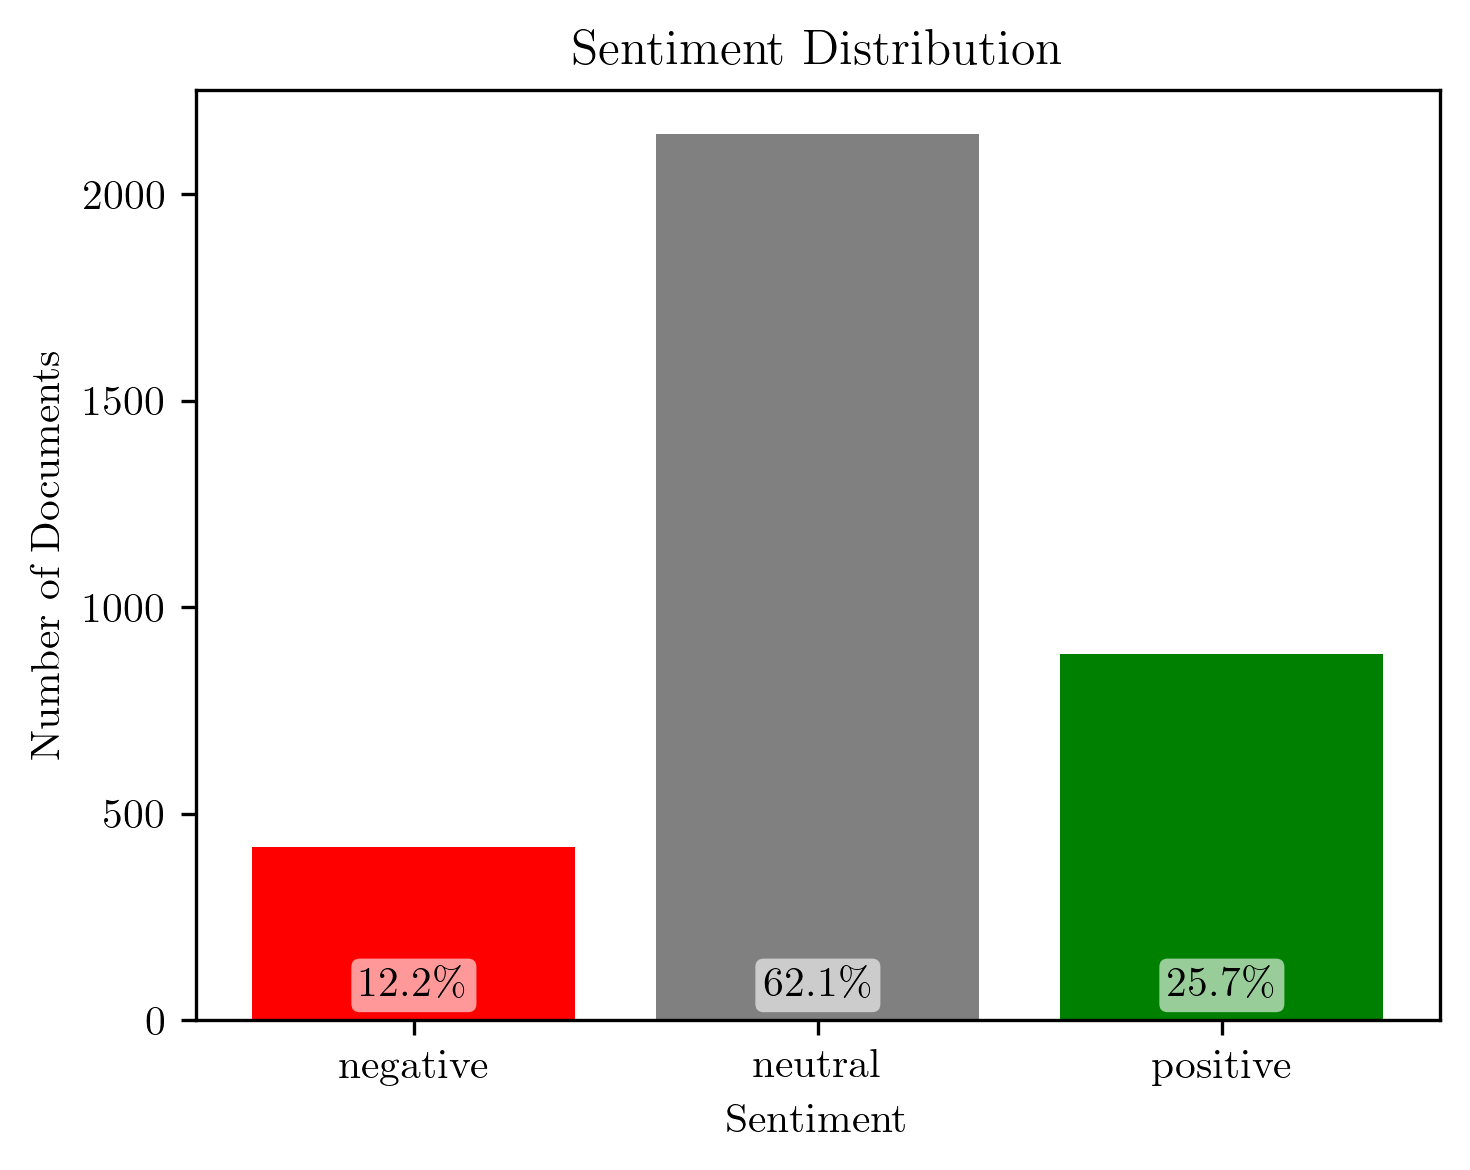
\includegraphics[width=1\linewidth]{assets/sentiment_distribution.png}
    \caption{Class distribution in the 75\% agreement dataset.}
    \label{fig:sentiment_distribution}
\end{figure}

The frequency distribution of document lengths helped determine the maximum number of tokens to use (considering the limit is 512 for BERT), as shown in Fig. \ref{fig:word_count_distribution}.

\begin{figure}[H]
    \centering
    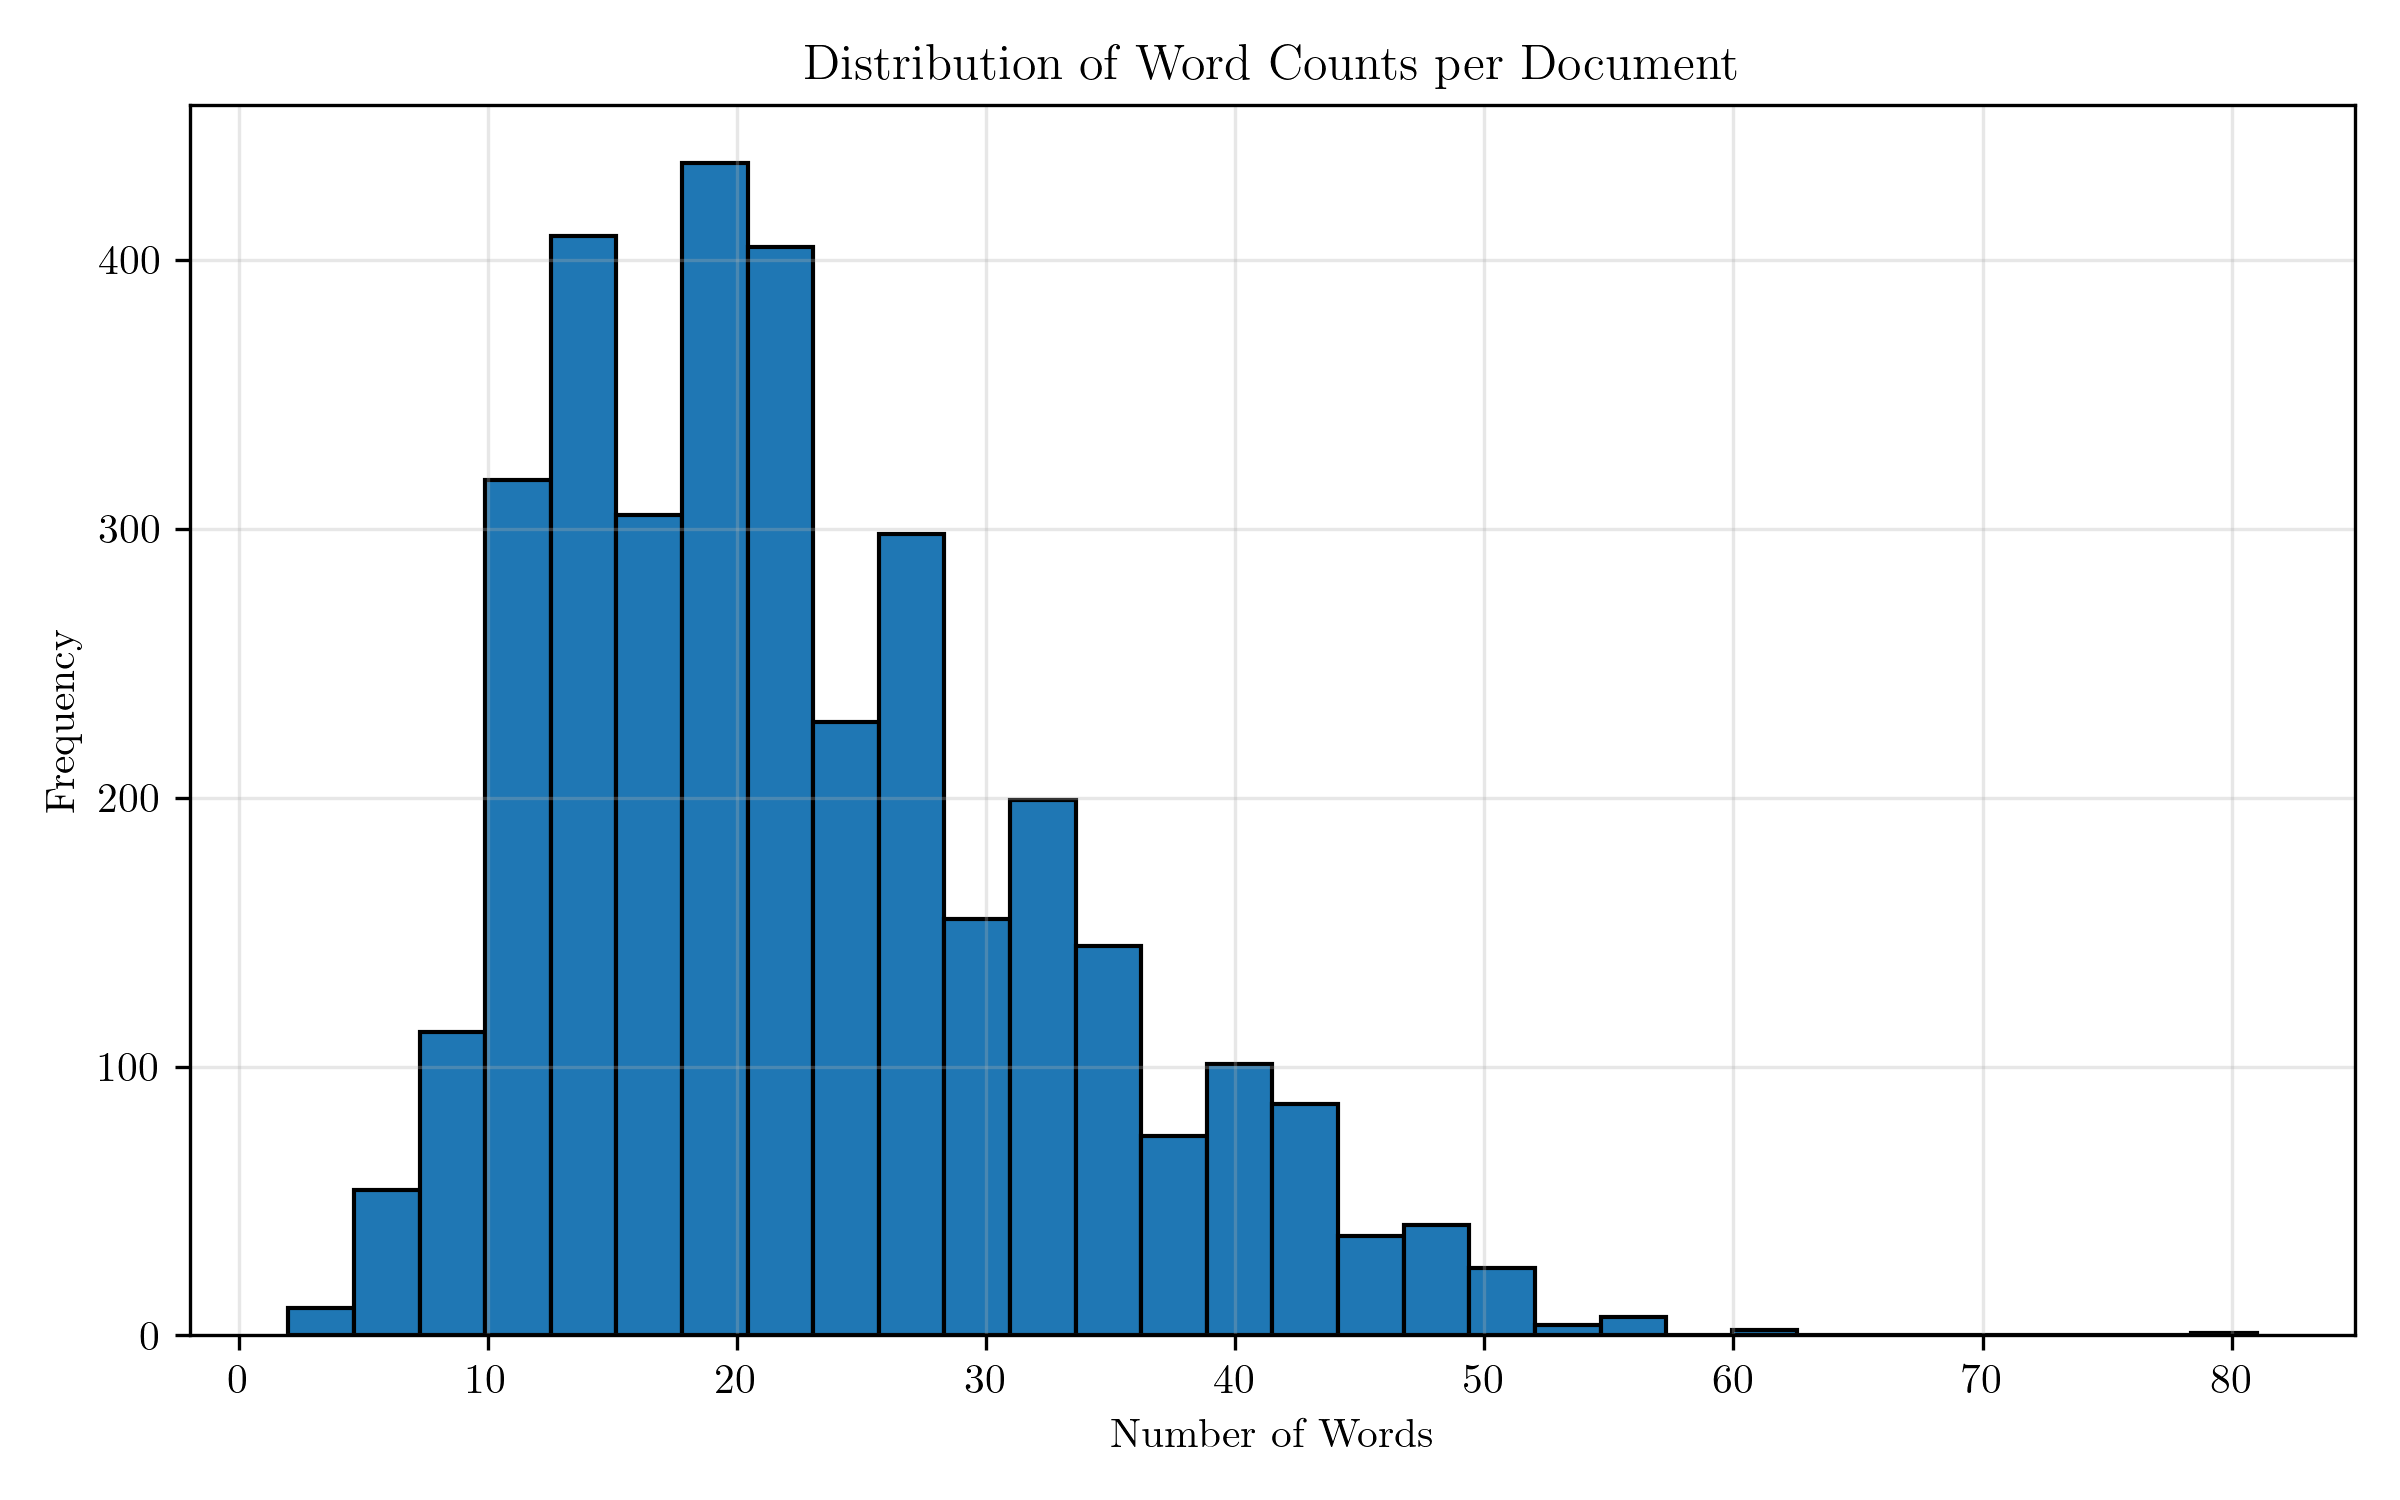
\includegraphics[width=1\linewidth]{assets/word_count_distribution.png}
    \caption{Word count distribution per document for the 75\% agreement dataset.}
    \label{fig:word_count_distribution}
\end{figure}

\begin{figure}[H]
    \centering
    
\includegraphics[width=1\linewidth]{assets/word_cloud_75agree.png}
    \caption{Most frequent words in the dataset, visualized as a word cloud.}
    \label{fig:word_cloud_75agree}
\end{figure}


%To identify words that are most indicative of sentiment class, word frequencies were compared across classes. Terms such as \textit{down}, \textit{decreased}, \textit{profit}, \textit{fell}, and \textit{rose} showed significantly higher frequency in specific sentiment categories, making them particularly relevant for classification.

Figure \ref{fig:word_cloud_75agree} shows a word cloud with the most frequent words in the dataset subset with 75\% annotator agreement, highlighting key terms that dominate the financial news domain. To identify words most indicative of sentiment class, word frequencies were then compared across sentiment categories. Terms such as \textit{down}, \textit{decreased}, \textit{profit}, \textit{fell}, and \textit{rose} appeared with significantly higher frequency in specific classes, making them particularly relevant for classification.

\subsection{Preprocessing}

The selected dataset (75\% agreement) was split 80/20 for training/testing.
The testing dataset was unique, meaning that all the sentences present in this subset were removed from any other dataset (of all the possible agreement levels), to prevent data leakage.

%The preprocessing changed slightly between models, and is adequately detailed in their section. The preprocessing here mentioned was carried before any model training.

The preprocessing changed slightly between models and is detailed in the corresponding sections. The preprocessing described here was performed prior to any model training, as was the class balance mentioned earlier.

\subsection{Model Evaluation and Validation Strategy}

Prior to model training, 5-fold cross-validation was performed for hyperparameter tuning, followed by training on the full dataset. Models were continuously evaluated using learning curves and comparative metrics such as the confusion matrix, F1-score, and accuracy.

\section{Model Architectures: LSTM, FastText, and BERT}

With the maining goal of classifying the sentiment of sentences, we have selected three models for an initial assessment, and proceeded with more complex iterations on the best model. The final model was further developed with data augmentation, and weighted classes, that will be further detailed below. The models selected were: Long Short-Term Memory (LSTM), fastText, and Bidirectional Encoder Representations from Transformers (BERT).

\subsubsection{Long Short-Term Memory}

LSTM is a type of recurrent neural network (RNN), introduced by Hochreiter and Schmidhuber (1997). Its architecture was designed to solve the vanishing gradient problem common in standard RNNs by introducing memory cells and gating mechanisms (input, output, and forget gates) to retain long term dependencies in sequential data, such as time series or sentences. In the present work, a standard LSTM architecture was used, without pre-training.

\subsubsection{fastText}

Developed by Joulin \textit{et al.} at Facebook AI (2016), fastText is built on the Word2Vec (word representation in a vectorial space) and extended it by incorporating subword information. Rather than representing each word as a single entity, it breaks it down to character n-grams. This allows to represent sentences by averaging word embeddings, making it very lightweight and fast to train on large datasets, with minimal tuning. The lightweightness and little tunability makes it less differenciate and harder to adapt to specific cases. In the present study, the standard supervised fastText implementation was used for sentence classification, without pre-trained embeddings.

\subsubsection{Bidirectional Encoder Representations from Transformers}

BERT was introduced by Devlin \textit{et al.} and colleagues at Google (2018), and is a deep-transformer model pre-trained on large corpora using masked language modeling (hiding one word in the sentence for the model to predict) and next sentence prediction. BERT is capable of considering both forwards and backwards dependencies with a word, simultaneously. This allows for much better understanding of nuanced language patterns and semantics. Despite the higher computational requirements, it still is manageable at a local level, and benefits heavily from fine-tuning for specific NLP tasks. In this work, the \texttt{bert-base-uncased} variant was used as the base model.

\subsection{Initial Benchmark}

The initial models went through rounds of 5-fold cross validation, with the hyperparameter search spaces as indicated in Table \ref{tab:basemodel_hyp}.

\begin{table}[H]
    \caption{Hyperparameter search space and selected values for the initial models.}
    \centering
    \label{tab:basemodel_hyp}
    \begin{subtable}[t]{0.45\textwidth}
        \centering
        \begin{tabular}{lll}
        \toprule
        \textbf{Hyperparameter} \phantom{a} & \textbf{Search Space} \phantom{aha} & \textbf{Selected Value} \\
        \midrule
        Epochs & $\{20, 21, \ldots, 99\}$ & 88 \\
        Learning rate & $[10^{-5}, 10^{-2}]$ & $4\times10^{-3}$ \\
        Embedding dimension & $\{100, 200, 300\}$ & 200 \\
        \bottomrule
        \end{tabular}
        \vspace{.3em}
        \caption{fastText hyperparameters.}
        \label{parameters_basefasttext}
        \vspace{.1em}
    \end{subtable}

    \begin{subtable}[t]{0.45\textwidth}
        \centering
        \begin{tabular}{lll}
        \toprule
        \textbf{Hyperparameter} & \textbf{Search Space} & \textbf{Selected Value} \\
        \midrule
        Epochs & $\{2, 3, 5, 8, 10, 15\}$ & 3 \\
        Learning rate & $[10^{-5}, 10^{-3}]$ & $10^{-4}$ \\
        Embedding dimension & $\{32, 64, 128, 256\}$ & 128 \\
        LSTM units & $\{32, 64, 128, 256\}$ & 32 \\
        Dropout & $[0, 0.5]$ & 0.2 \\
        Recurrent dropout & $[0, 0.5]$ & 0 \\
        \bottomrule
        \end{tabular}
        \vspace{.3em}
        \caption{LSTM hyperparameters.}
        \vspace{.1em}
        \label{parameters_baselstm}
    \end{subtable}

    \begin{subtable}[t]{0.45\textwidth}
        \centering
        \begin{tabular}{lll}
        \toprule
        \textbf{Hyperparameter} \phantom{aaah} & \textbf{Search Space} \phantom{aaa} & \textbf{Selected Value} \\
        \midrule
        Epochs & $\{1,2,3,4,5\}$ & 2 \\
        Learning rate & $[10^{-5}, 10^{-2}]$ & $10^{-4}$ \\
        Weight decay & $[0, 0.5]$ & 0.1 \\
        \bottomrule
        \end{tabular}
        \vspace{.3em}
        \caption{BERT hyperparameters.}
        \label{parameters_basebert}
    \end{subtable}
\end{table}

After fitting the models with the best hyperparameters, the models were trained on the complete training set, with the results in Table \ref{basemodel_models}.
\begin{table}[H]
\centering
\caption{Initial benchmark metric results across the models for both the training and test sets.}
\label{basemodel_models}
\begin{tabular}{lcccc}
\toprule
\textbf{Model} & \multicolumn{2}{c}{\textbf{Accuracy}} & \multicolumn{2}{c}{\textbf{F1 (macro)}} \\
\cmidrule(lr){2-3} \cmidrule(lr){4-5}
 & \textbf{Train} & \textbf{Test} & \textbf{Train} & \textbf{Test} \\
\midrule
fastText & 0.54 & 0.65 & 0.45 & 0.44 \\
LSTM & 0.67 & 0.66 & 0.63 & 0.63 \\
BERT & 0.97 & 0.92 & 0.97 & 0.91 \\
\bottomrule
\end{tabular}
\end{table}

From the results, there is a clear gap between the models, with BERT performing best, followed by LSTM and fastText. These findings align with the literature, although LSTM can achieve better performance when using bi-LSTM. However, the purpose here was to evaluate \textit{vanilla} models as an initial assessment.

Given BERT's superior performance, it was selected for more detailed analysis and further experimentation, with its evaluation metrics and class-wise error distribution examined below. From this point onward, this model is referred to as B-BERT. 

From the learning curve (Fig. \ref{fig:base_bert_learning_curve}) the model seems to learn well, albeit the validation loss does increase slightly towards the end, overlapping the training curve.

\begin{figure}[H]
    \centering
    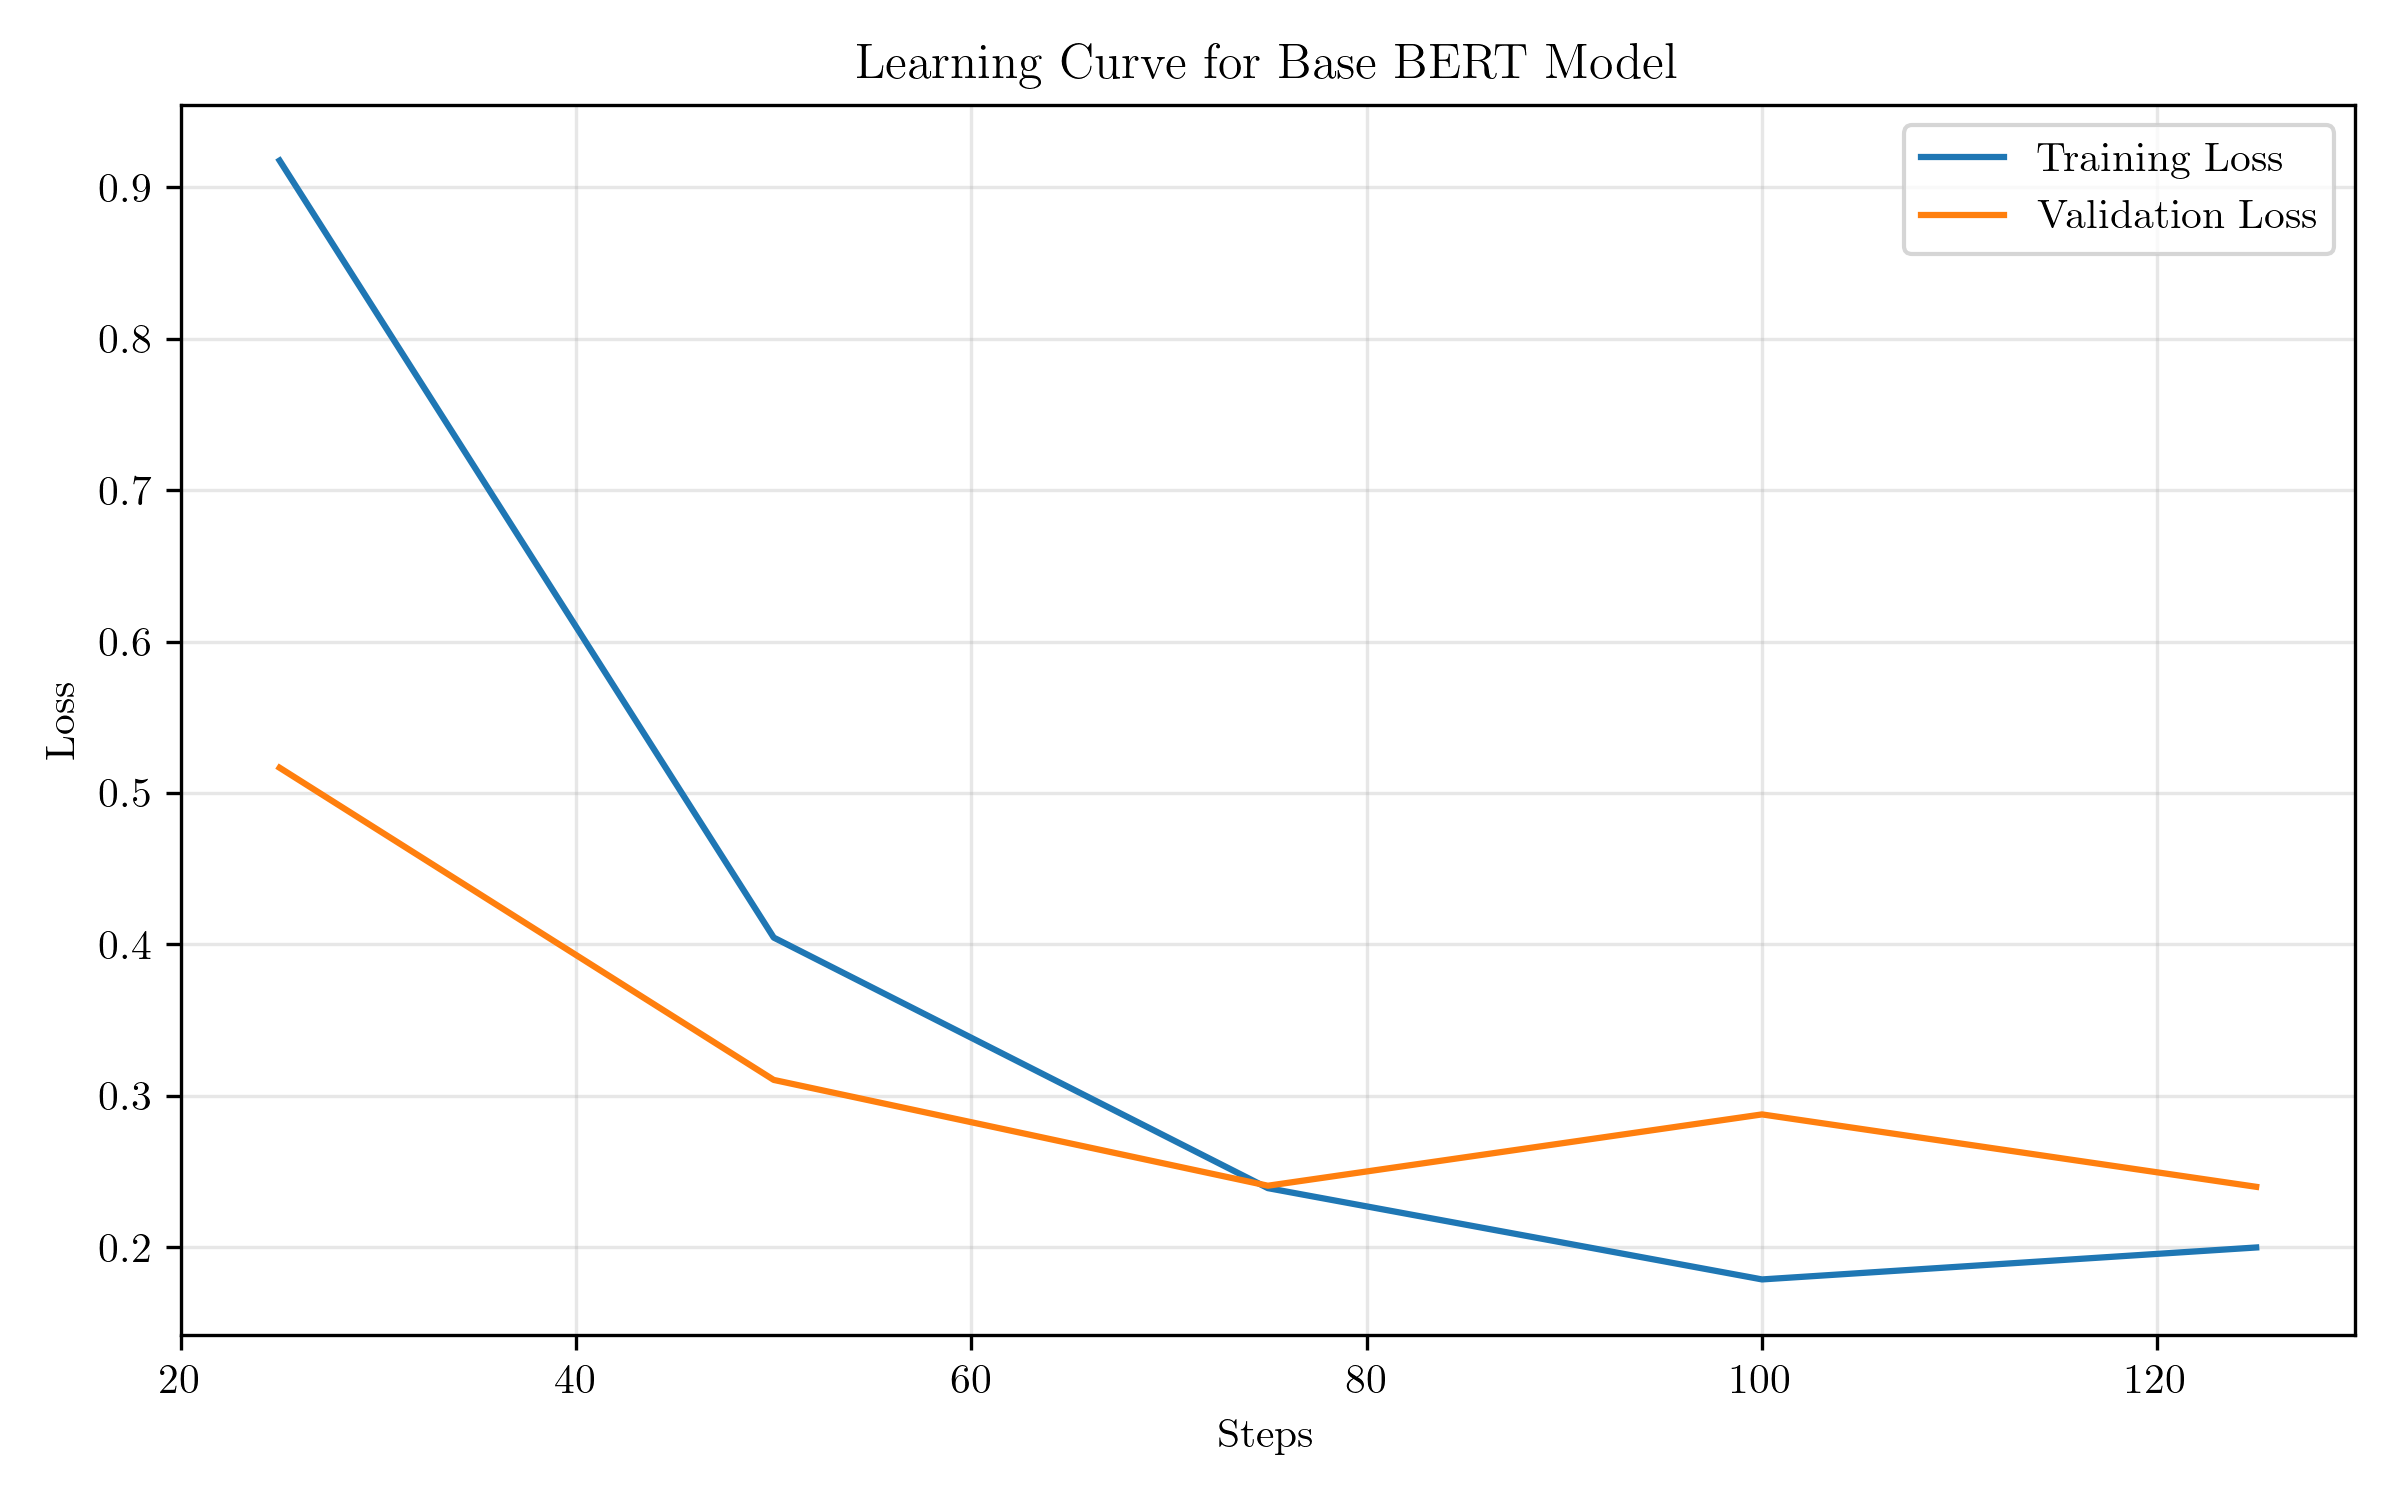
\includegraphics[width=1\linewidth]{assets/base_bert_learning_curve.png}
    \caption{B-BERT learning curve.}
    \label{fig:base_bert_learning_curve}
\end{figure}

From the confusion matrix and training metrics (Fig. \ref{fig:base_bert_confusion_matrix_Train} and Table \ref{cr_basebert_train}), the model seems to learn well, with no class suffering in particular in terms of performance. 

\begin{figure}[H]
    \centering
    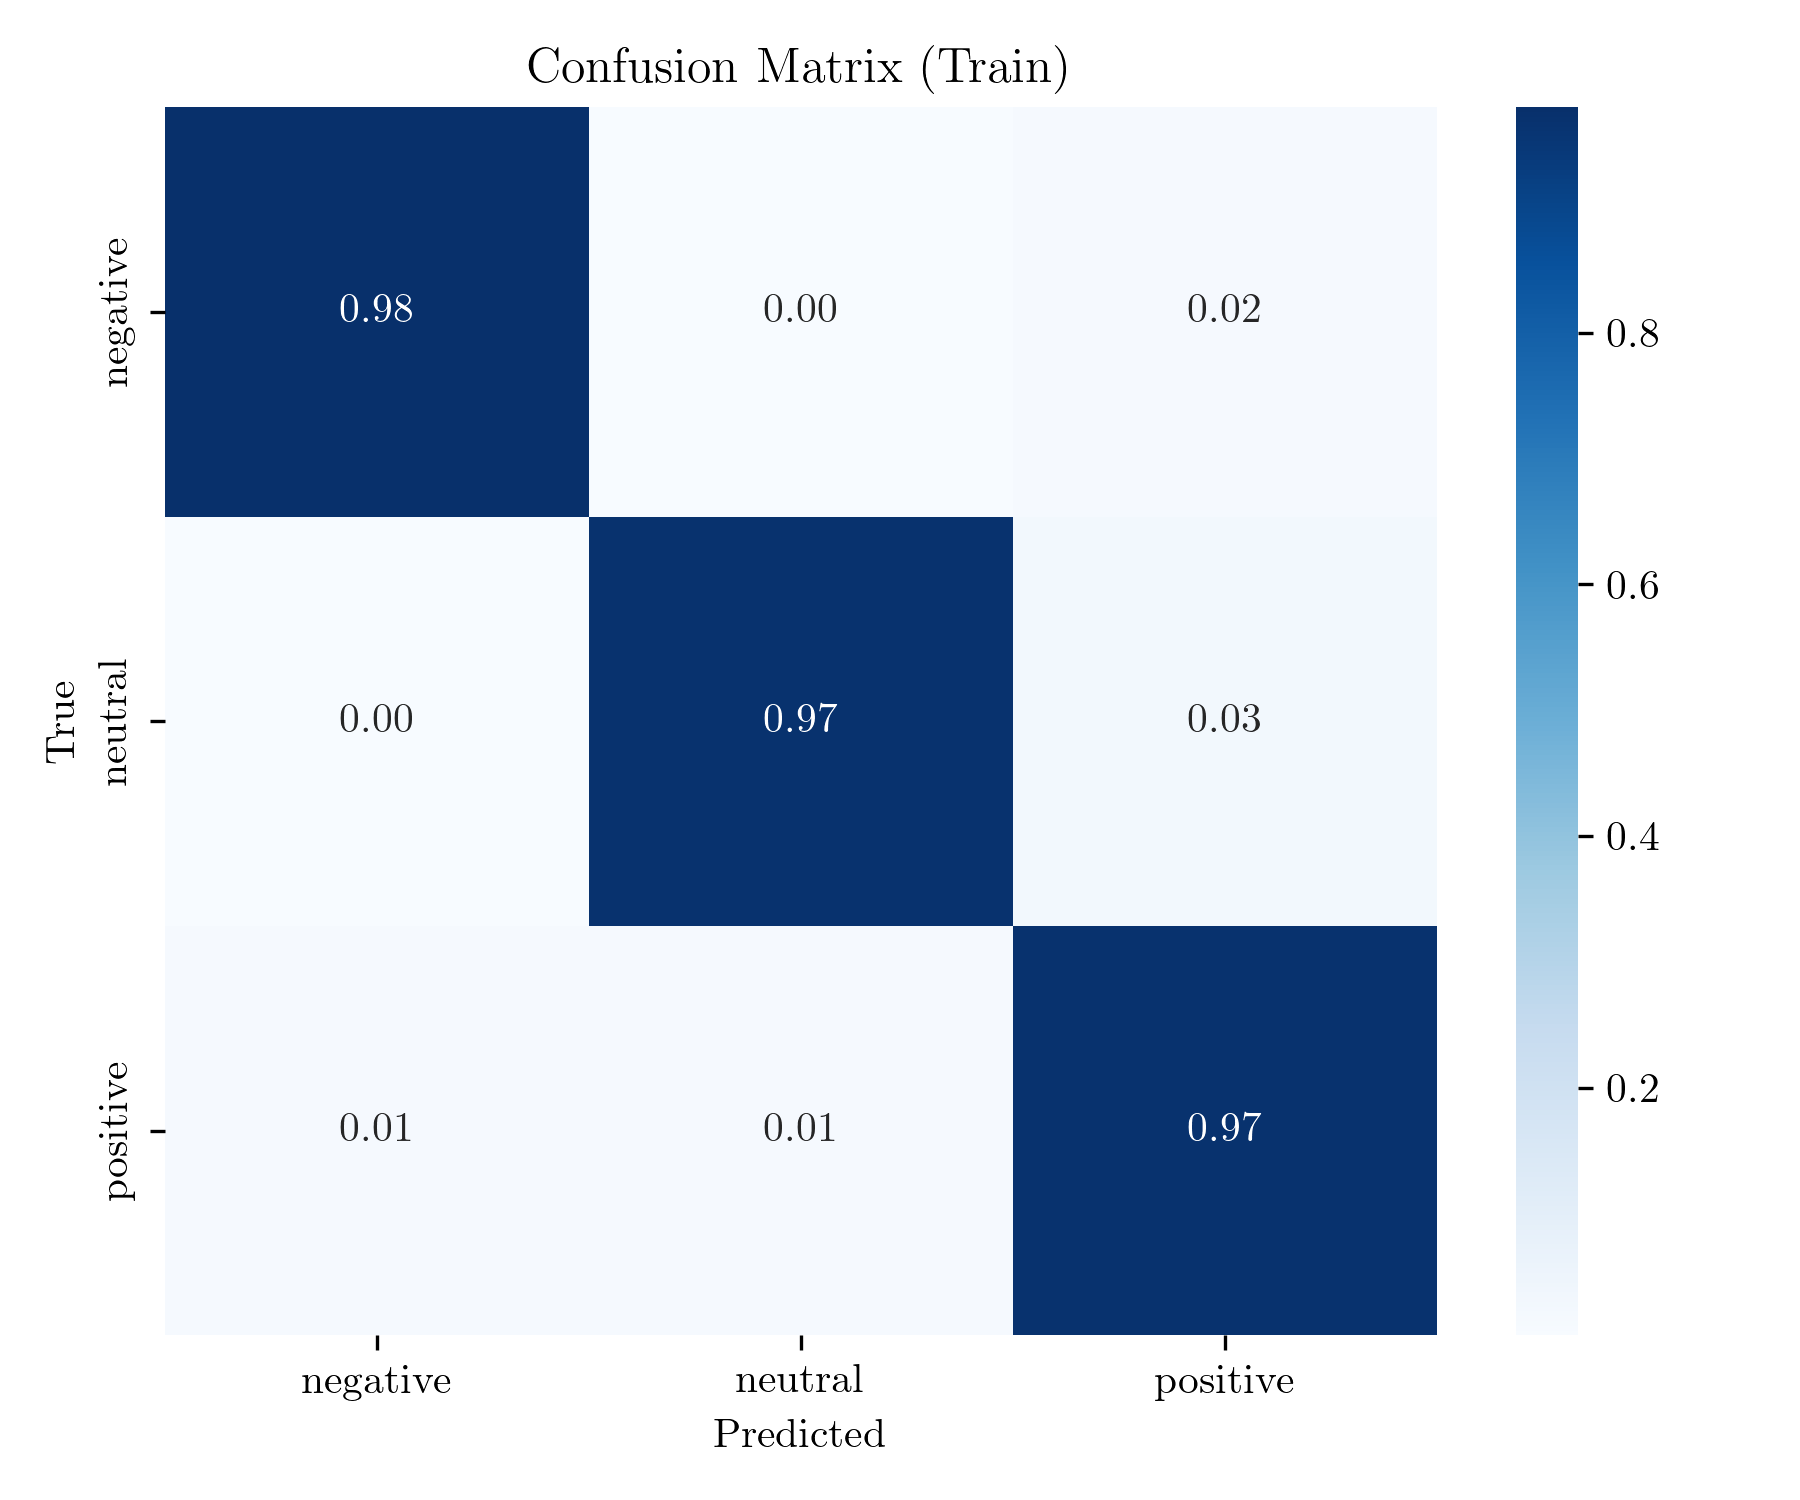
\includegraphics[width=1\linewidth]{assets/base_bert_confusion_matrix_Train.png}
    \caption{Normalized confusion matrix for the training set with the B-BERT model.}
    \label{fig:base_bert_confusion_matrix_Train}
\end{figure}

\begin{table}[H]
\centering
\caption{Classification report for B-BERT on training data.}
\label{cr_basebert_train}
\begin{tabular}{lcccccc}
\toprule
\textbf{Class} & \textbf{Precision} & \textbf{Recall} & \textbf{F1-Score} & \textbf{Support} \\
\midrule
Negative & 0.98 & 0.98 & 0.98 & 336 \\
Neutral & 0.98 & 0.97 & 0.98 & 336 \\
Positive & 0.96 & 0.97 & 0.96 & 336 \\
\midrule
\textbf{Accuracy} &  &  & 0.97 & 1008 \\
\textbf{Macro avg} & 0.97 & 0.97 & 0.97 & 1008 \\
\textbf{Weighted avg} & 0.97 & 0.97 & 0.97 & 1008 \\
\bottomrule
\end{tabular}
\end{table}

From the test results (Fig.~\ref{fig:base_bert_confusion_matrix_Test} and Table~\ref{cr_basebert_test}), the model appears to be overfit, showing difficulties in generalizing and achieving performance comparable to the training set, with the macro average being significantly lower.

\begin{figure}[H]
    \centering
    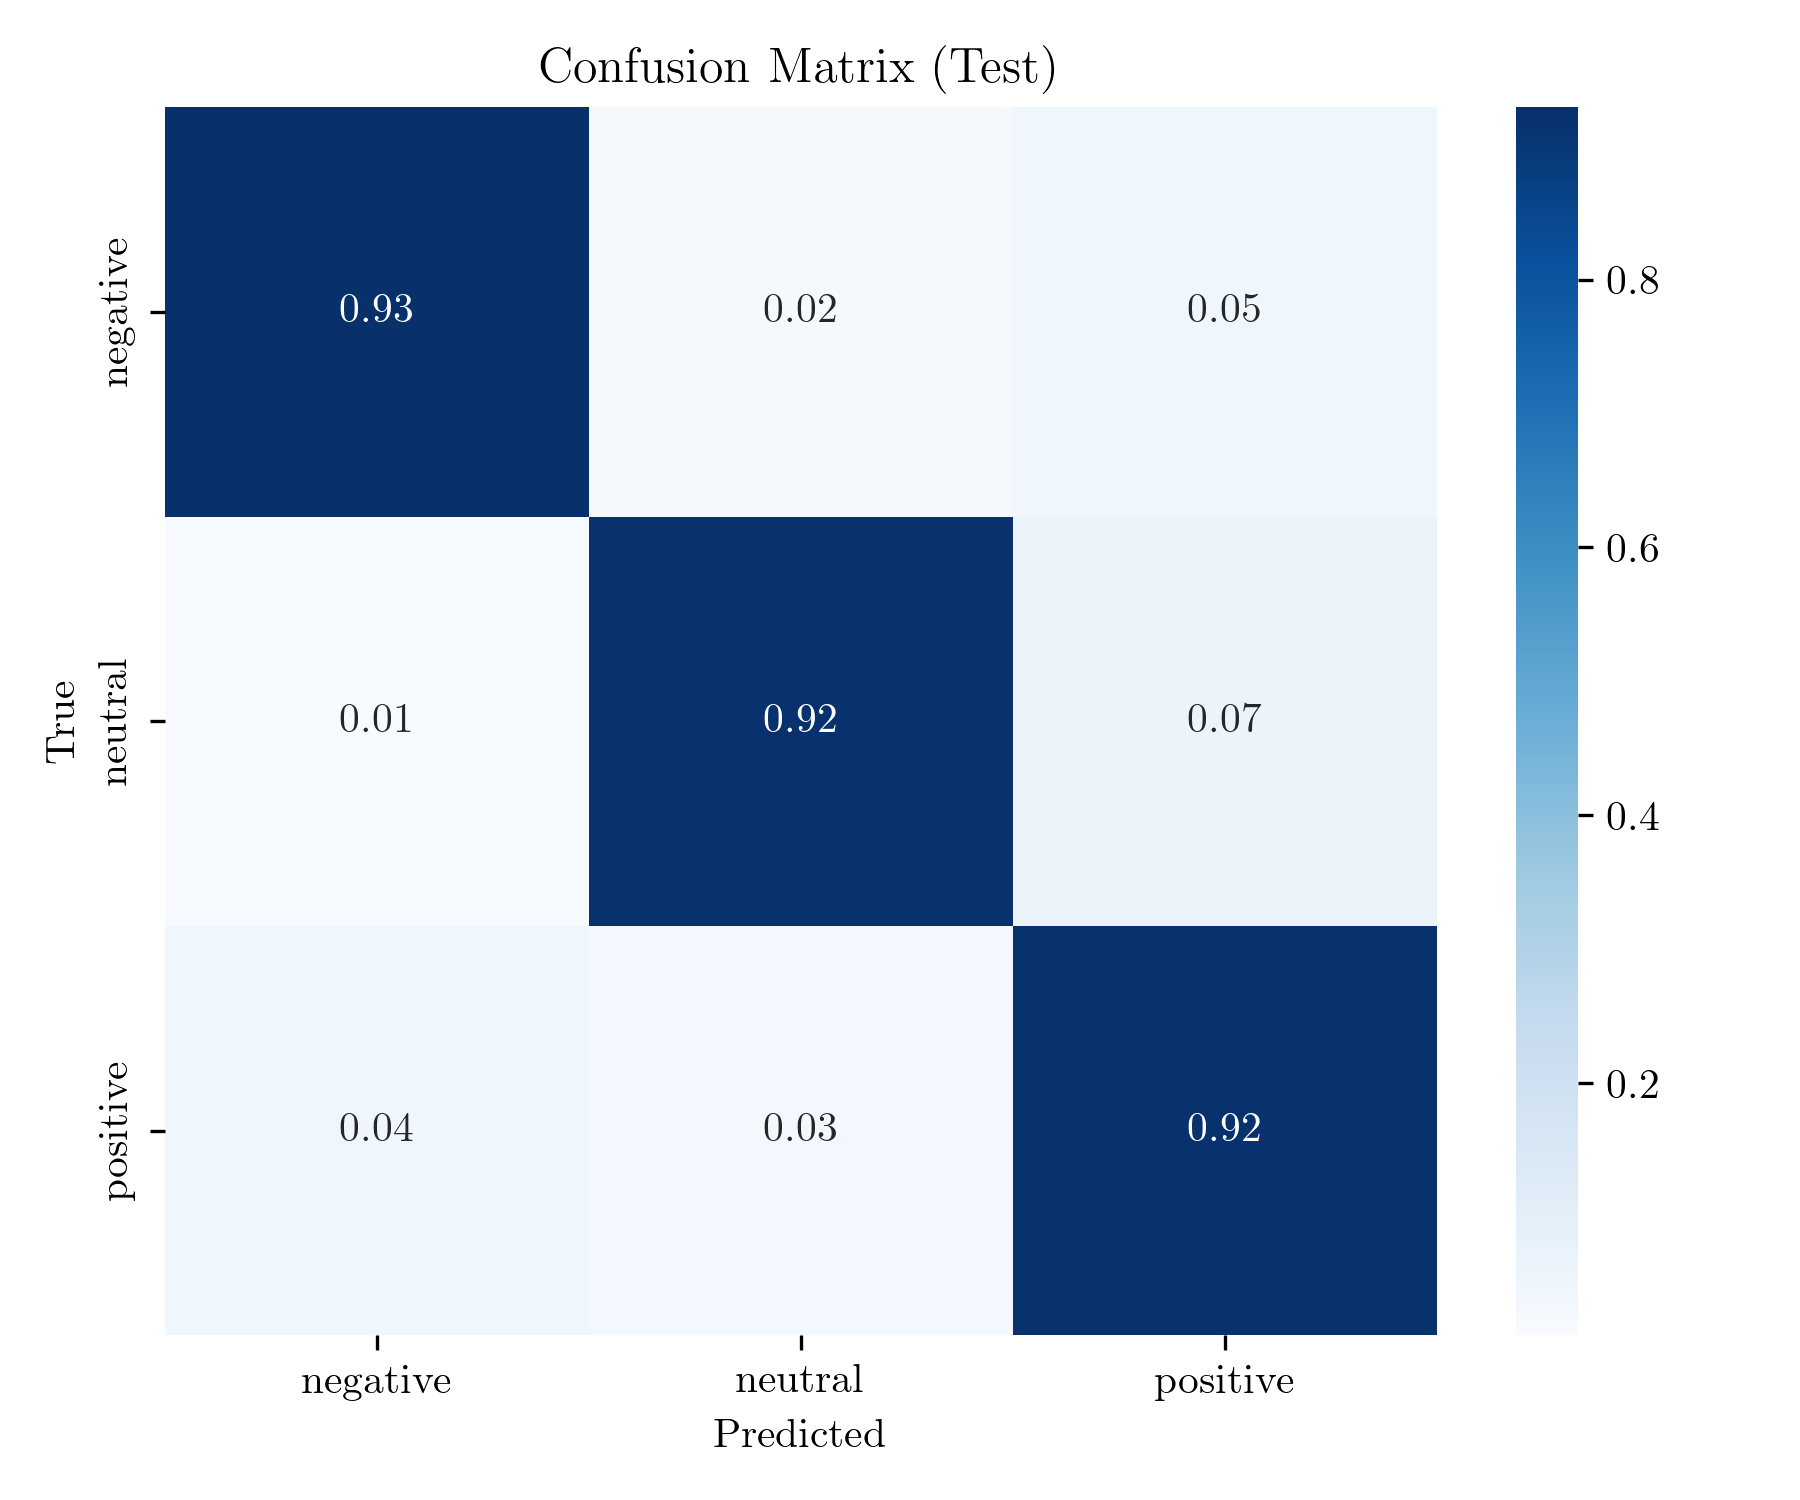
\includegraphics[width=1\linewidth]{assets/base_bert_confusion_matrix_Test.png}
    \caption{Normalized confusion matrix for the test set with the B-BERT model.}
    \label{fig:base_bert_confusion_matrix_Test}
\end{figure}

\begin{table}[H]
\centering
\caption{Classification report for B-BERT on test data.}
\label{cr_basebert_test}
\begin{tabular}{lcccccc}
\toprule
\textbf{Class} & \textbf{Precision} & \textbf{Recall} & \textbf{F1-Score} & \textbf{Support} \\
\midrule
Negative & 0.86 & 0.93 & 0.89 & 84 \\
Neutral & 0.98 & 0.92 & 0.95 & 429 \\
Positive & 0.84 & 0.92 & 0.88 & 178 \\
\midrule
\textbf{Accuracy} &  &  & 0.92 & 691 \\
\textbf{Macro avg} & 0.89 & 0.92 & 0.91 & 691 \\
\textbf{Weighted avg} & 0.93 & 0.92 & 0.92 & 691 \\
\bottomrule
\end{tabular}
\end{table}

\subsection{Data Augmented Model - DA-BERT}

To improve the model's generalization capability, an online data augmentation strategy was implemented, consisting of back-translation (translation-based augmentation using intermediate pivoting paraphrasing, English to German and back), lexical substitution (where random words are replaced with WordNet-based synonyms), and template-based augmentation (by using named entity recognition, the identified words are replaced with template tokens such as ORG or DATE to generalize the sentence). Some examples of this augmentation are available in Table \ref{tab:fpb_augm_examples}.

\begin{table}[ht]
\centering
\caption{Example sentences from the Financial PhraseBank and their augmented examples.}
\label{tab:fpb_augm_examples}
\begin{tabular}{p{3.5cm}p{3.5cm}}
\toprule
\textbf{Original} & \textbf{Augmented} \\
\midrule
In the building and home improvement trade, sales decreased by 22.5\% to EUR 201.4 mn. & In the building and DIY trade, sales decreased by 22.5\% to EUR 201.4 million. \\
In January–June 2010, diluted loss per share stood at EUR 0.3 versus EUR 0.1 in the first half of 2009. & In the first half of 2009, diluted loss per share stood at EUR 0.3 versus EUR 0.1 in the same period of 2008. \\
\bottomrule
\end{tabular}
\end{table}

The cross-validation procedure mentioned previously was executed, with the search space and selected values indicated in Table \ref{parameters_basebert}.

\begin{table}[H]
\centering
\caption{Hyperparameter search space for DA-BERT and selected values after fine-tuning.}
\label{parameters_basebert}
\begin{tabular}{lll}
\toprule
\textbf{Hyperparameter} & \textbf{Search Space} & \textbf{Selected Value} \\
\midrule
Epochs & $\{1,2,3,4,5\}$ & 2 \\
Learning rate & $[10^{-5}, 10^{-2}]$ & $10^{-4}$ \\
Weight decay & $[0, 0.5]$ & 0.1 \\
\bottomrule
\end{tabular}
\end{table}

%With this, the model was trained on the full training set, and from the learning curve (Fig. \ref{fig:data_augmented_bert_learninc_curve}) we can see the model was capable of generalizing well throughout the training routine, with validation increasing slightly between the $50^{\textnormal{th}}$ and $80^{\textnormal{th}}$ steps, but then following the downward trend to the end of the training, without early stopping (considering the number of epochs was included in the CV procedure, this was expected).

With this setup, the model was trained on the full training set, using the same online data augmentation pipeline. As shown in the learning curve (Fig. \ref{fig:data_augmented_bert_learninc_curve}), the model was able to generalize well throughout the training routine, with validation performance slightly increasing between the $50^{\textnormal{th}}$ and $80^{\textnormal{th}}$ steps, then following a downward trend toward the end. Although the curve does not exhibit a stable or horizontal convergence, this behavior is due to an implicit early stopping effect governed by the number of epochs, which was treated as a hyperparameter during fine-tuning.

\begin{figure}[H]
    \centering
    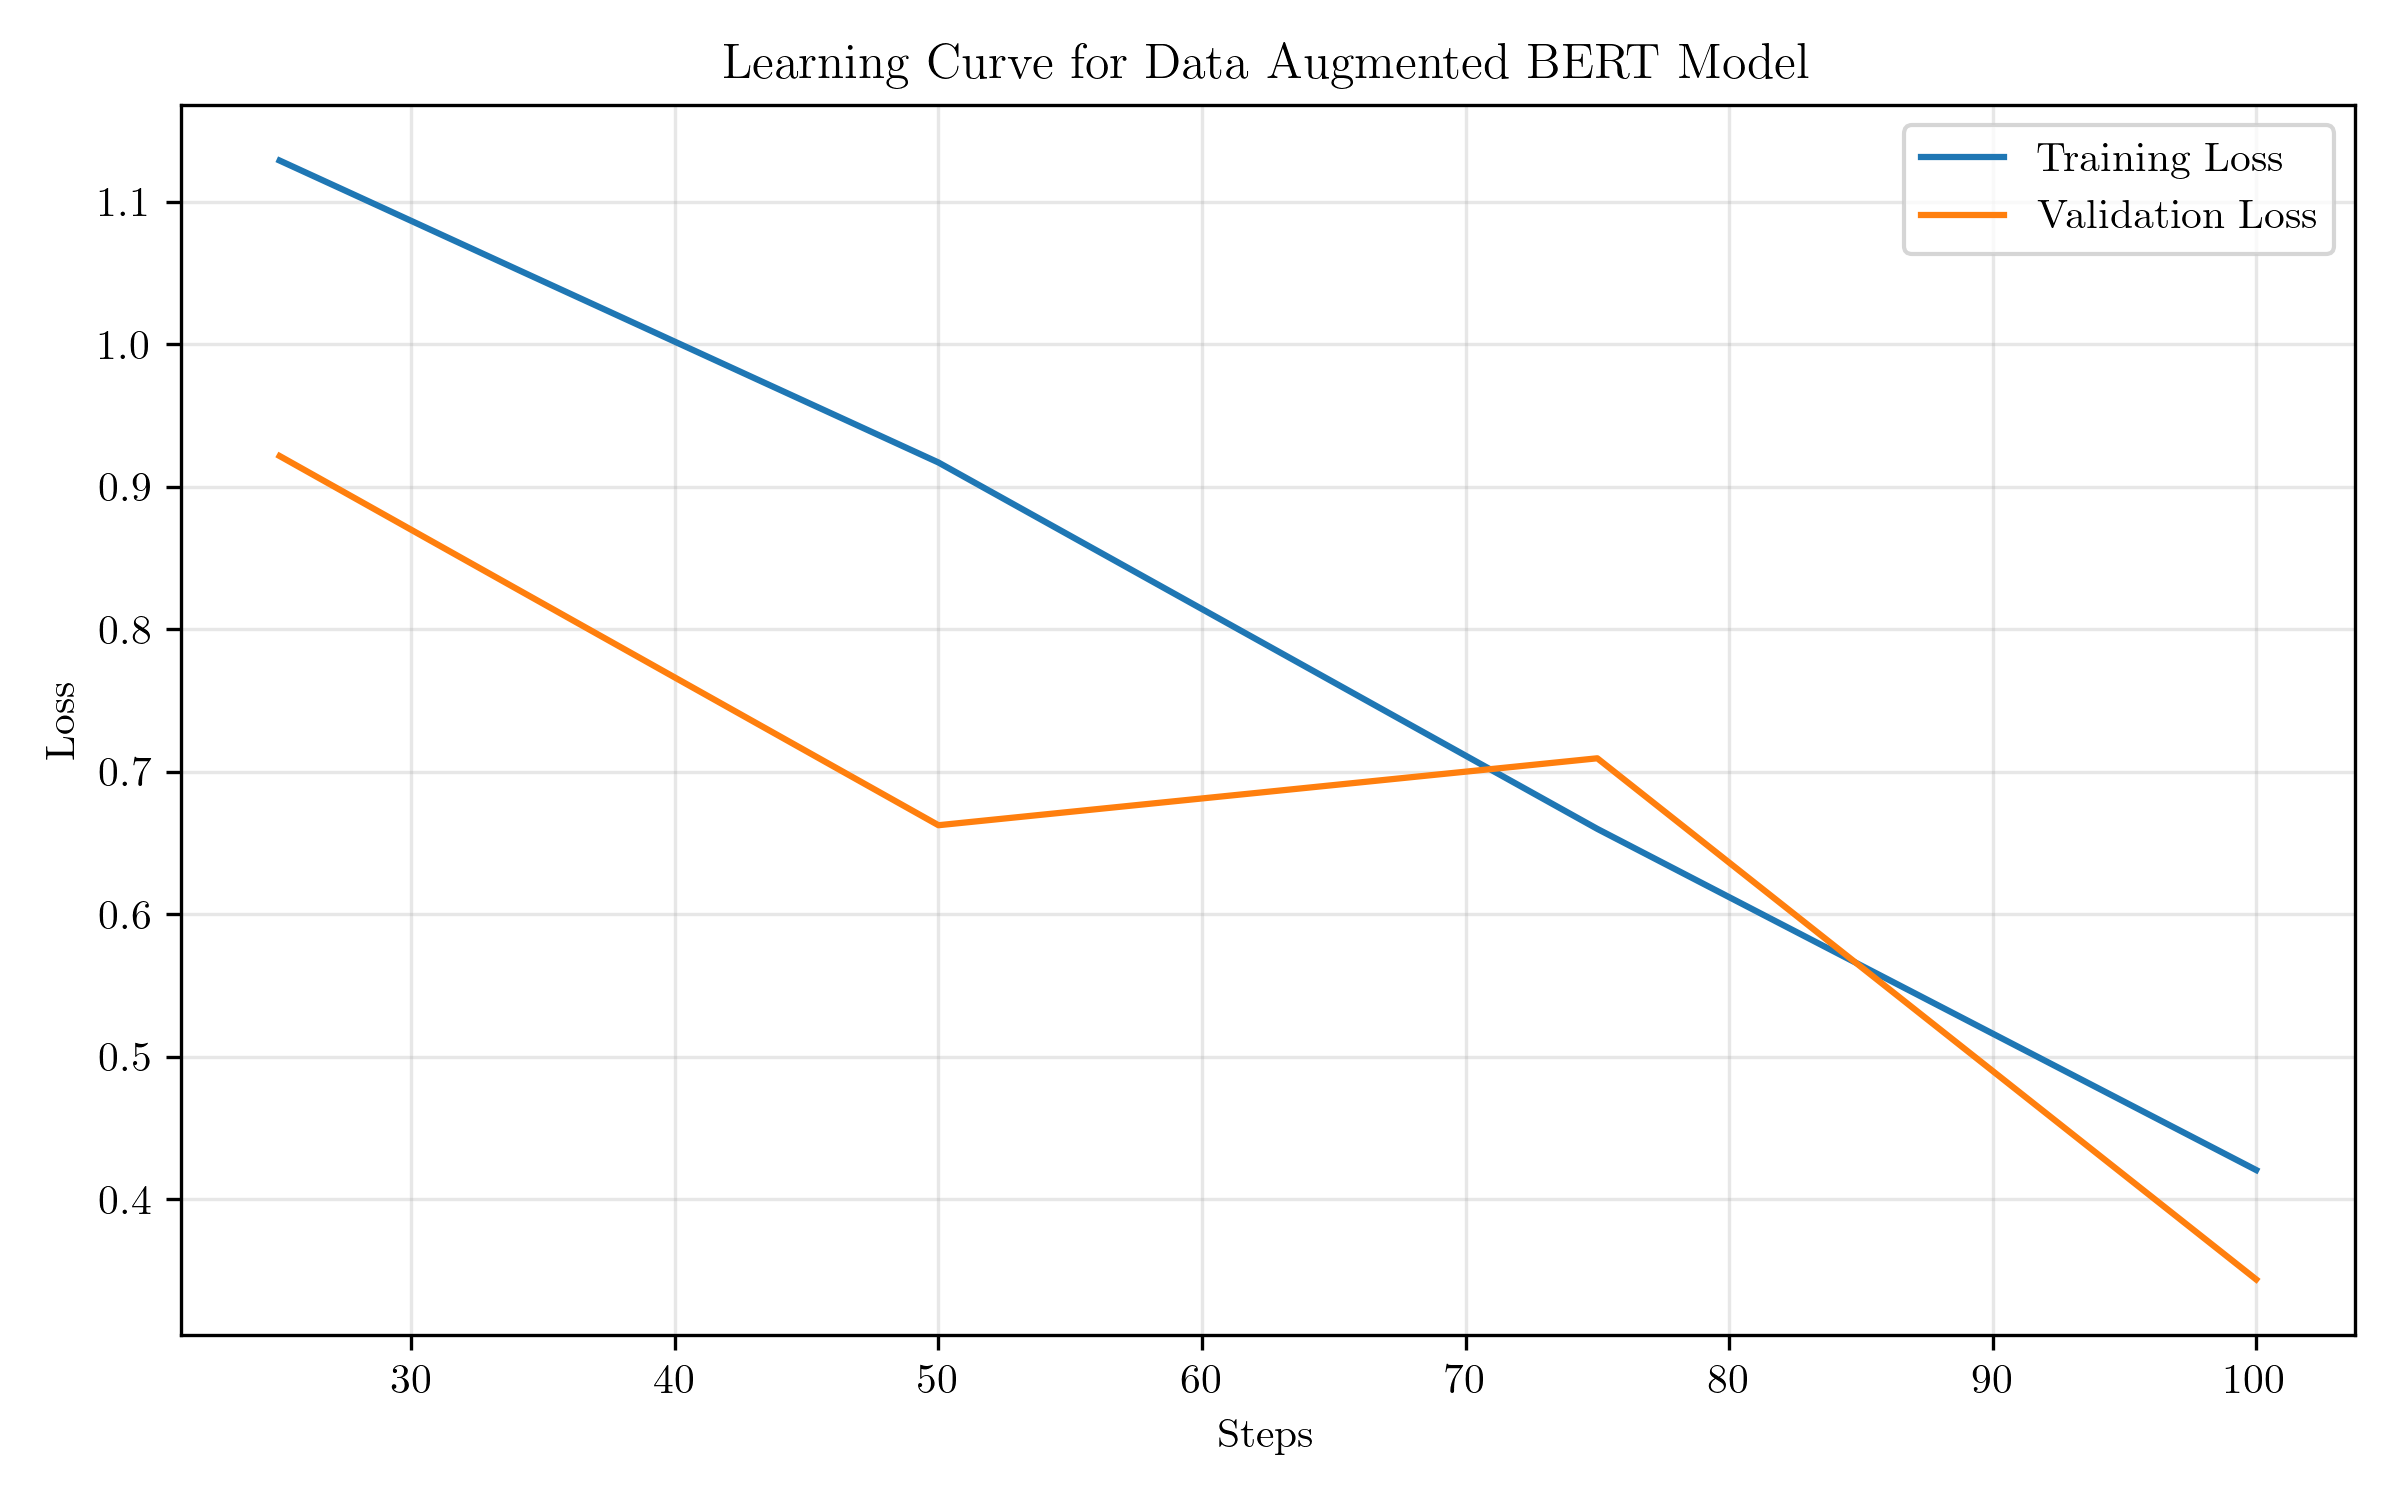
\includegraphics[width=1\linewidth]{assets/data_augmented_bert_learninc_curve.png}
    \caption{DA-BERT learning curve.}
    \label{fig:data_augmented_bert_learninc_curve}
\end{figure}

The confusion matrix from the training (Fig. \ref{fig:dataaugmented_bert_confusion_matrix_Train}) shows that the model performed well, but slightly worse in particular for the \textit{Positive} class, which can also be confirmed from the classification report (Table \ref{cr_augmbert_train}), where the recall is considerably lower. The overall metrics (accuracy, macro average, and weighted average) indicate worse performance compared to the B-BERT model, though the comparison is not entirely fair given that B-BERT showed signs of overfitting.

\begin{figure}[H]
    \centering
    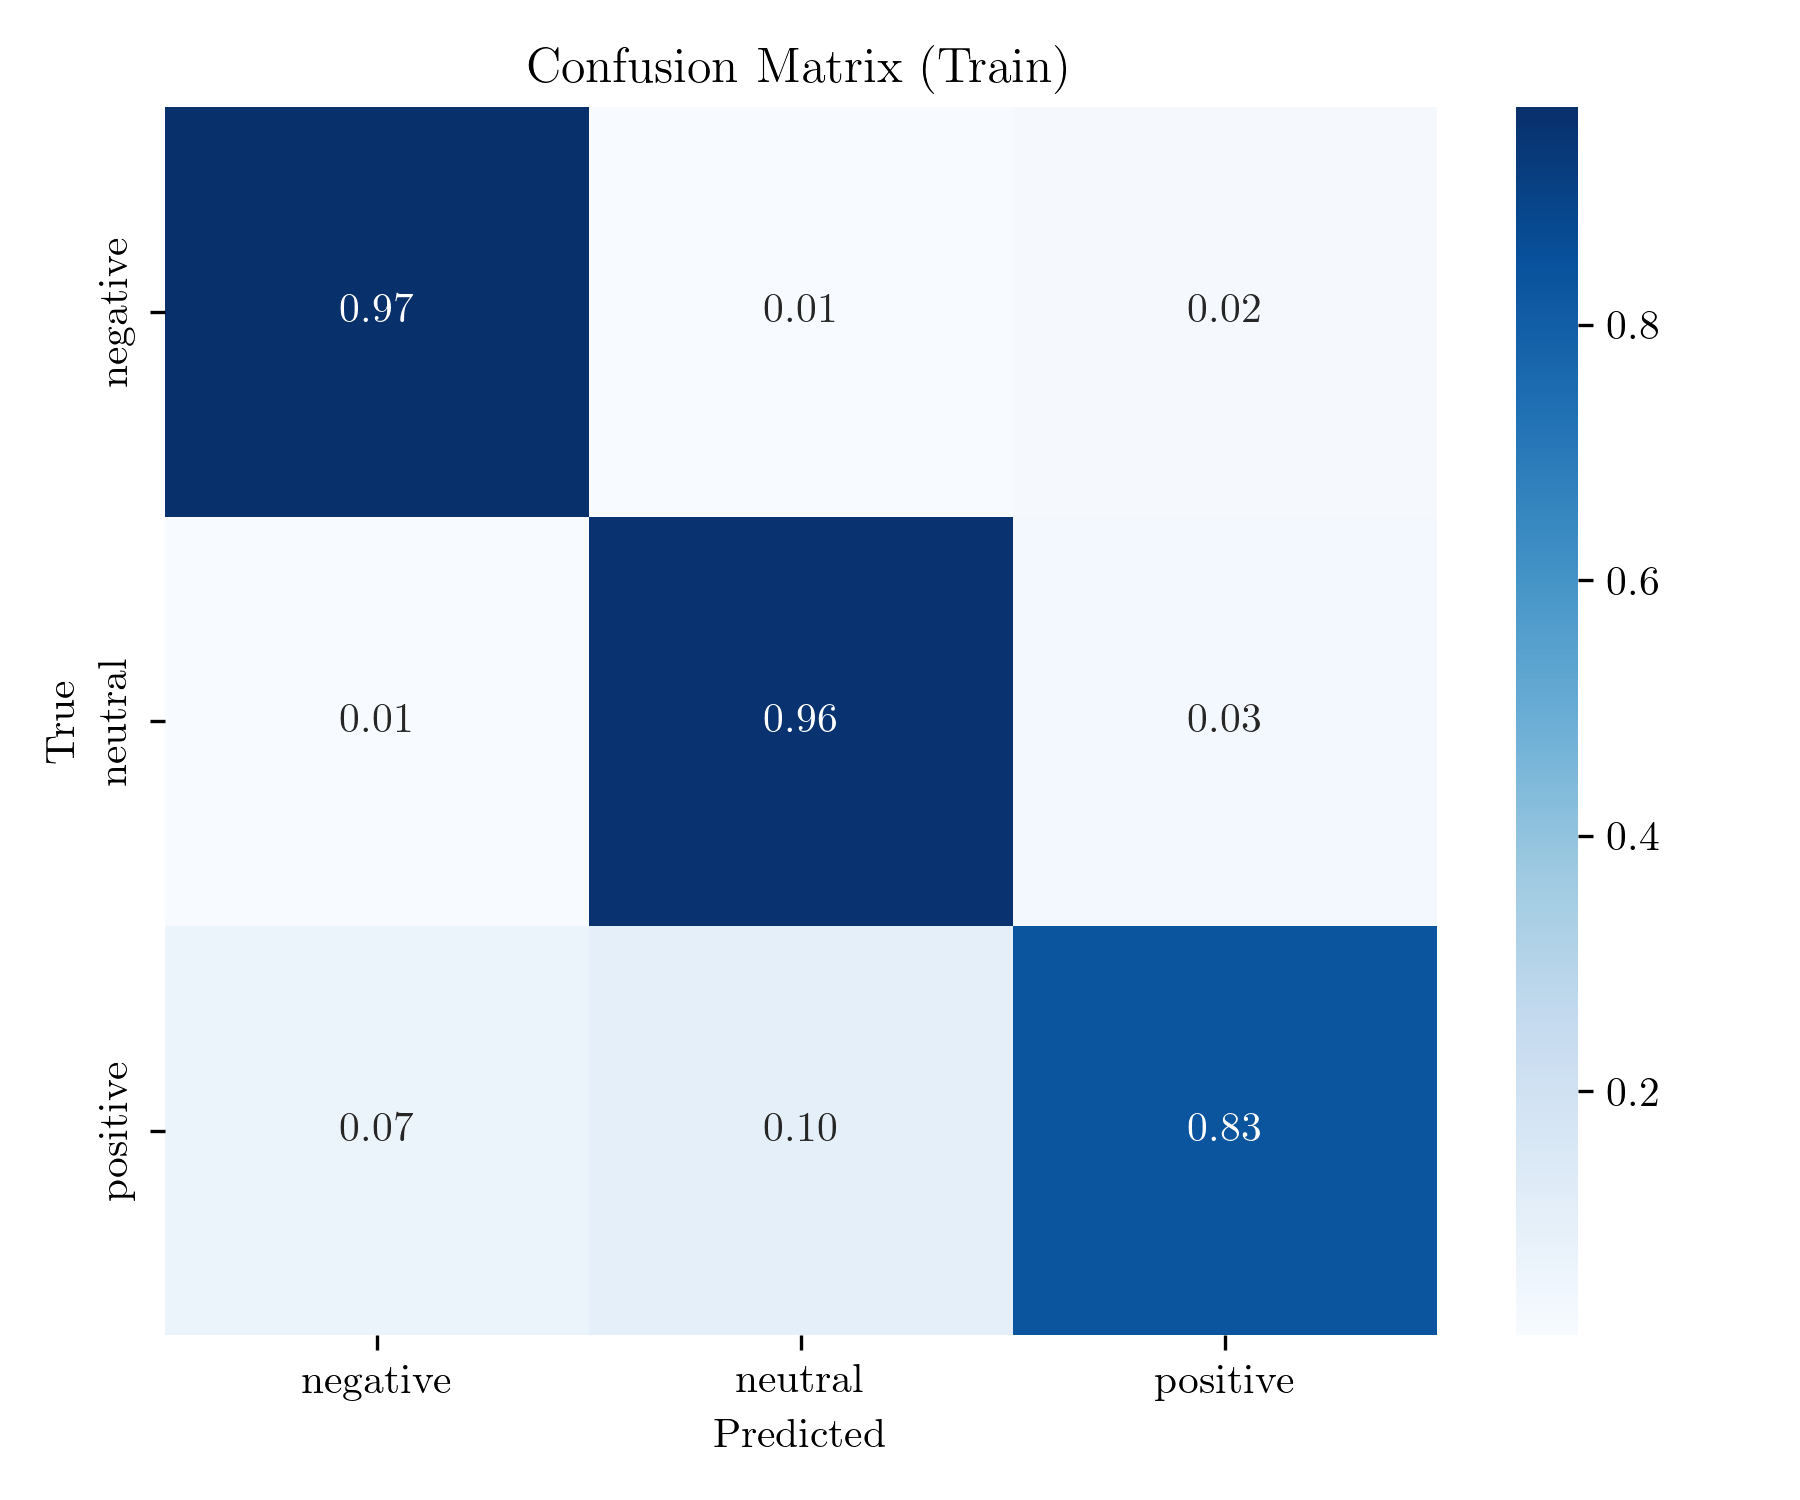
\includegraphics[width=1\linewidth]{assets/dataaugmented_bert_confusion_matrix_Train.png}
    \caption{Normalized confusion matrix for DA-BERT model on training data.}
    \label{fig:dataaugmented_bert_confusion_matrix_Train}
\end{figure}


\begin{table}[H]
\centering
\caption{Classification report for DA-BERT on training data.}
\label{cr_augmbert_train}
\begin{tabular}{lcccccc}
\toprule
\textbf{Class} & \textbf{Precision} & \textbf{Recall} & \textbf{F1-Score} & \textbf{Support} \\
\midrule
Negative & 0.92 & 0.97 & 0.95 & 336 \\
Neutral & 0.90 & 0.96 & 0.93 & 336 \\
Positive & 0.94 & 0.83 & 0.88 & 336 \\
\midrule
\textbf{Accuracy} &  &  & 0.92 & 1008 \\
\textbf{Macro avg} & 0.92 & 0.92 & 0.92 & 1008 \\
\textbf{Weighted avg} & 0.92 & 0.92 & 0.92 & 1008 \\
\bottomrule
\end{tabular}
\end{table}

From the test confusion matrix (Fig. \ref{fig:dataaugmented_bert_confusion_matrix_Test}) there is a slight decrease for the \textit{Negative} and \textit{Neutral} classes, whereas the \textit{Positive} class keeps as is. The trend is confirmed from the classification report (Table \ref{cr_augmbert_test}), showing slightly worse metrics than for the training data.
%If your augmentation produces inputs that deviate too far from the real distribution (especially test-time distribution), the model learns artifacts that do not transfer. Example: if you apply aggressive paraphrasing, BERT may learn to rely on patterns not present in real test inputs.

\begin{figure}[H]
    \centering
    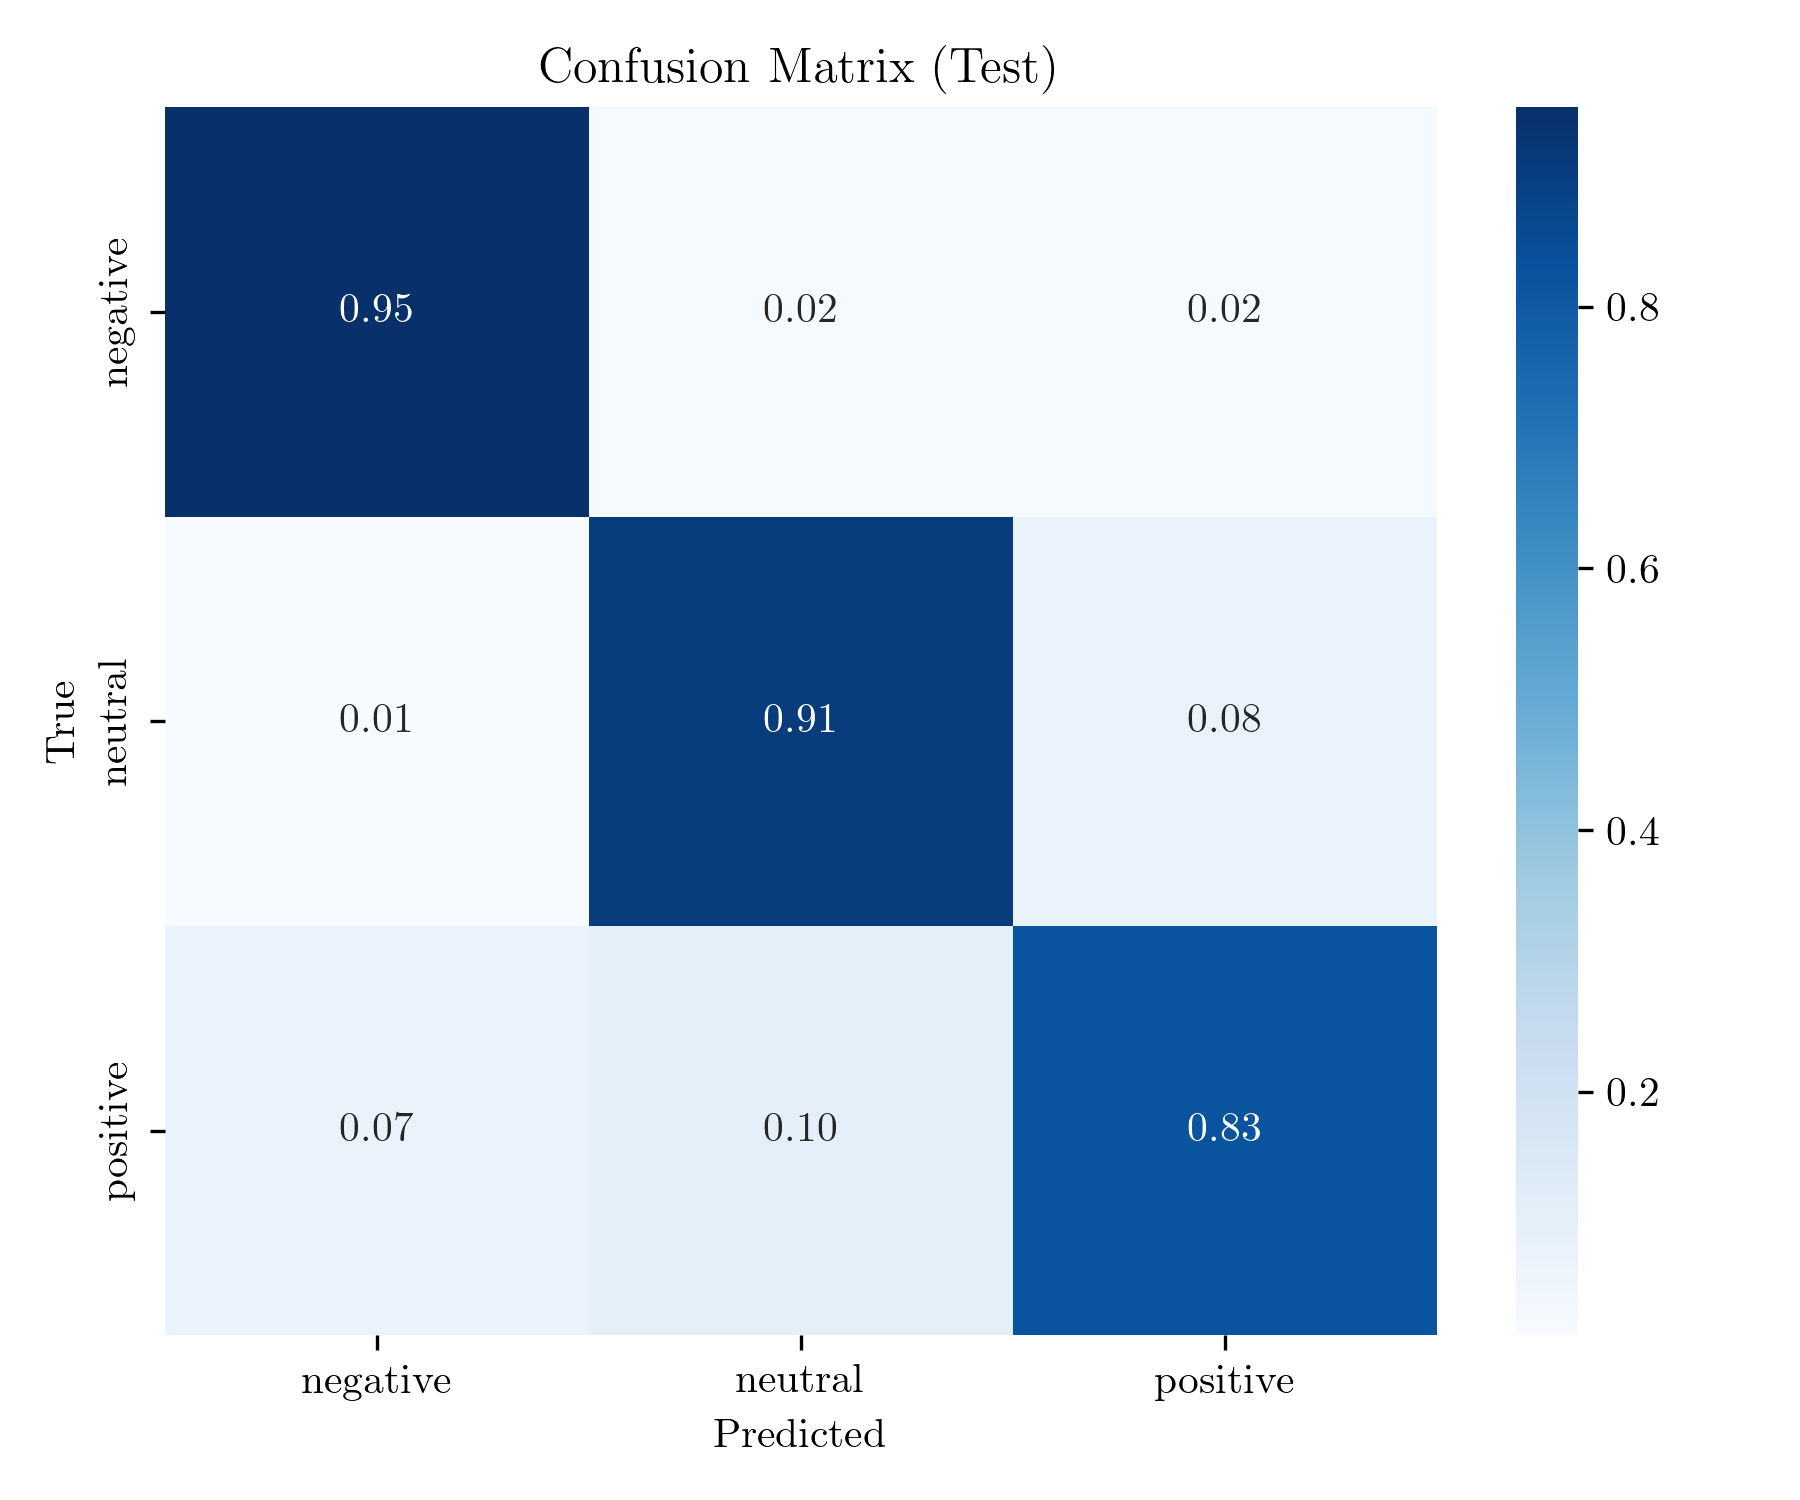
\includegraphics[width=1\linewidth]{assets/dataaugmented_bert_confusion_matrix_Test.png}
    \caption{Normalized confusion matrix for DA-BERT model on test data.}
    \label{fig:dataaugmented_bert_confusion_matrix_Test}
\end{figure}

\begin{table}[H]
\centering
\caption{Classification report for DA-BERT on test data.}
\label{cr_augmbert_test}
\begin{tabular}{lcccccc}
\toprule
\textbf{Class} & \textbf{Precision} & \textbf{Recall} & \textbf{F1-Score} & \textbf{Support} \\
\midrule
Negative & 0.81 & 0.95 & 0.87 & 84 \\
Neutral & 0.95 & 0.91 & 0.93 & 429 \\
Positive & 0.80 & 0.83 & 0.81 & 178 \\
\midrule
\textbf{Accuracy} &  &  & 0.89 & 691 \\
\textbf{Macro avg} & 0.85 & 0.89 & 0.87 & 691 \\
\textbf{Weighted avg} & 0.90 & 0.89 & 0.89 & 691 \\
\bottomrule
\end{tabular}
\end{table}

The model seems to be well fit, despite slight differences between training and test metrics. These can be explained given the data augmentation pipeline, that pushes the model towards generalization, while losing more obvious patterns that are kept in the undisturbed test set. 

\subsection{Instance Weighted Model - W-BERT}

For this model the approach aims to achieve a balance between quantity and quality of data. Rather than filtering documents based on the level of agreement, the goal was to introduce the level of agreement as penalty weights during training, with the model being more penalized for wrong classification of sentences with higher level of agreement and less so for the opposite cases.

After testing, the following formula was adopted for the agreement class weights, with $i \in \{50\%, 66\%, 75\%, 100\%\}$, where each value represents a level of annotator agreement associated with each sentence in the dataset.

$$
w_i = \text{scale} \cdot p_i = \left( \frac{N}{\sum_{j=1}^k n_j \cdot p_j} \right) \cdot  \left( \frac{e^{a_i}}{\sum_{j=1}^k e^{a_j}} \right) \text{,}
$$

\noindent where $a_i$ is the raw agreement scores for class $i$, $n_i$ the number of samples in class $i$, and $N$ the total number of instances.

The rationale behind this formulation starts from a set of empirically defined raw agreement scores, $a_i$, for each agreement class:

$$
\{0.50, 0.66, 0.75, 1.0\}
$$

These values represent the degree of annotator consensus and are transformed exponentially using the softmax function,

$$
p_i = \frac{e^{a_i}}{\sum_j e^{a_j}}
$$

\noindent to capture differences in confidence in a non-linear manner.

Following this transformation, a normalization factor is applied to account for agreement imbalance in the training dataset,

$$
\text{scale} = \frac{N}{\sum_i n_i \cdot p_i}
$$

\noindent ensuring that the average weight across all training instances equals 1, preserving the comparability of the loss function with a weightless scenario, such as the test dataset.

This approach leverages confidence information from agreement levels without distorting the overall loss scale during training.

Considering the dataset for this model, and accounting for class balance, the training dataset for this model had 520 observations per class, rather than the 336 from earlier. The hyperparameter search space and selected can be found in table \ref{parameters_wbert}.

\begin{table}[H]
\centering
\caption{Hyperparameter search space for W-BERT and selected values after fine-tuning.}
\label{parameters_wbert}
\begin{tabular}{lll}
\toprule
\textbf{Hyperparameter} & \textbf{Search Space} & \textbf{Selected Value} \\
\midrule
Epochs & $\{1, 2, 3, 4, 5\}$ & 3 \\
Learning rate & $[10^{-5}, 10^{-2}]$ & $10^{-4}$ \\
Weight decay & $[0, 0.5]$ & 0.1 \\
\bottomrule
\end{tabular}
\end{table}

The learning curve for the instance-weighted training loss and the weightless validation loss (Fig.~\ref{fig:weighted_bert_learning_curve}) shows that both training and validation losses decrease during the first half of training. Around the midpoint, the validation loss begins to increase slightly, while the training loss continues to decrease, indicating early signs of possible overfitting.

\begin{figure}[H]
    \centering
    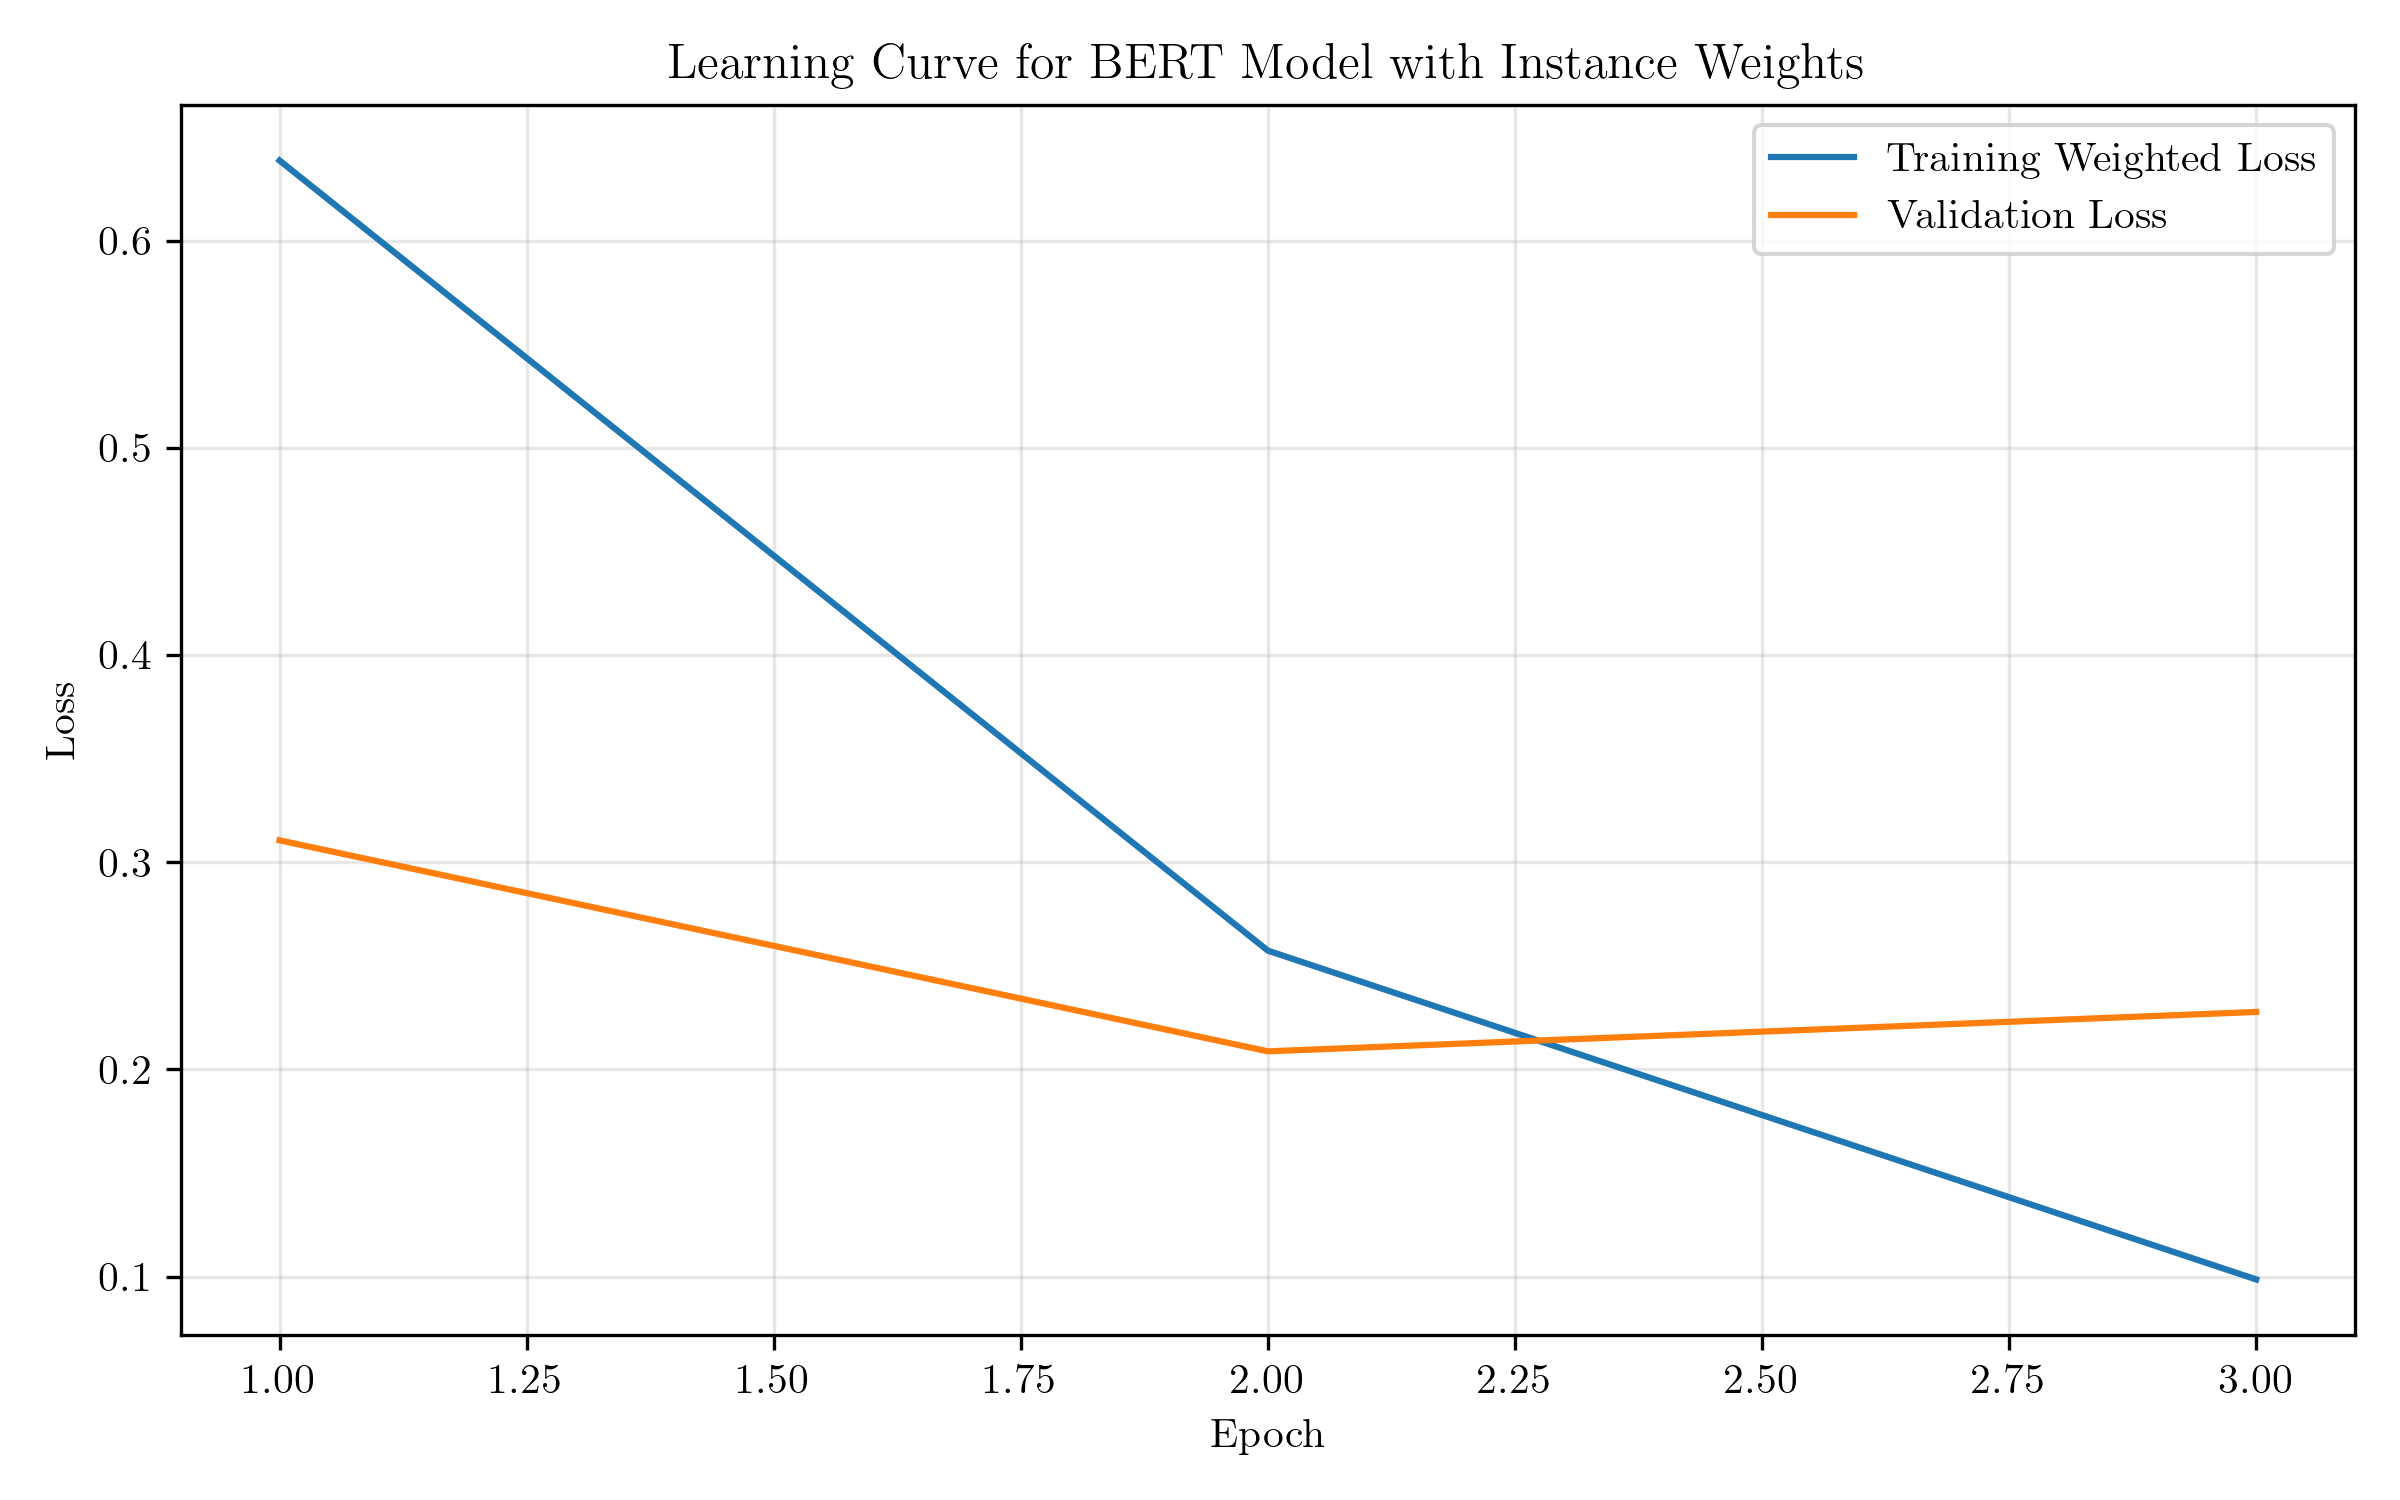
\includegraphics[width=1\linewidth]{assets/weighted_bert_learning_curve.png}
    \caption{W-BERT learning curve.}
    \label{fig:weighted_bert_learning_curve}
\end{figure}

For training metrics, only a portion of the training set was used, namely instances with at least 75\% agreement. This choice was motivated by the difficulty of incorporating instance weights into the calculation of certain metrics and the potential bias introduced if weighting is ignored. The 75\% agreement threshold was a natural selection, consistent with the threshold used throughout the study and for the test set.

The approach under analysis produced notable results. The confusion matrix for the partial training set (Fig. \ref{fig:weighted_bert_confusion_matrix_Partial}) and the classification report (Table \ref{cr_weightbert_train}) provide strong evidence that the model successfully learned to recognize the \textit{Negative} class. The improvement observed in the \textit{Positive} class supports the hypothesis that this category tends to exhibit lower annotator agreement, making it more difficult for models trained without weighting to capture.

\begin{figure}[H]
    \centering
    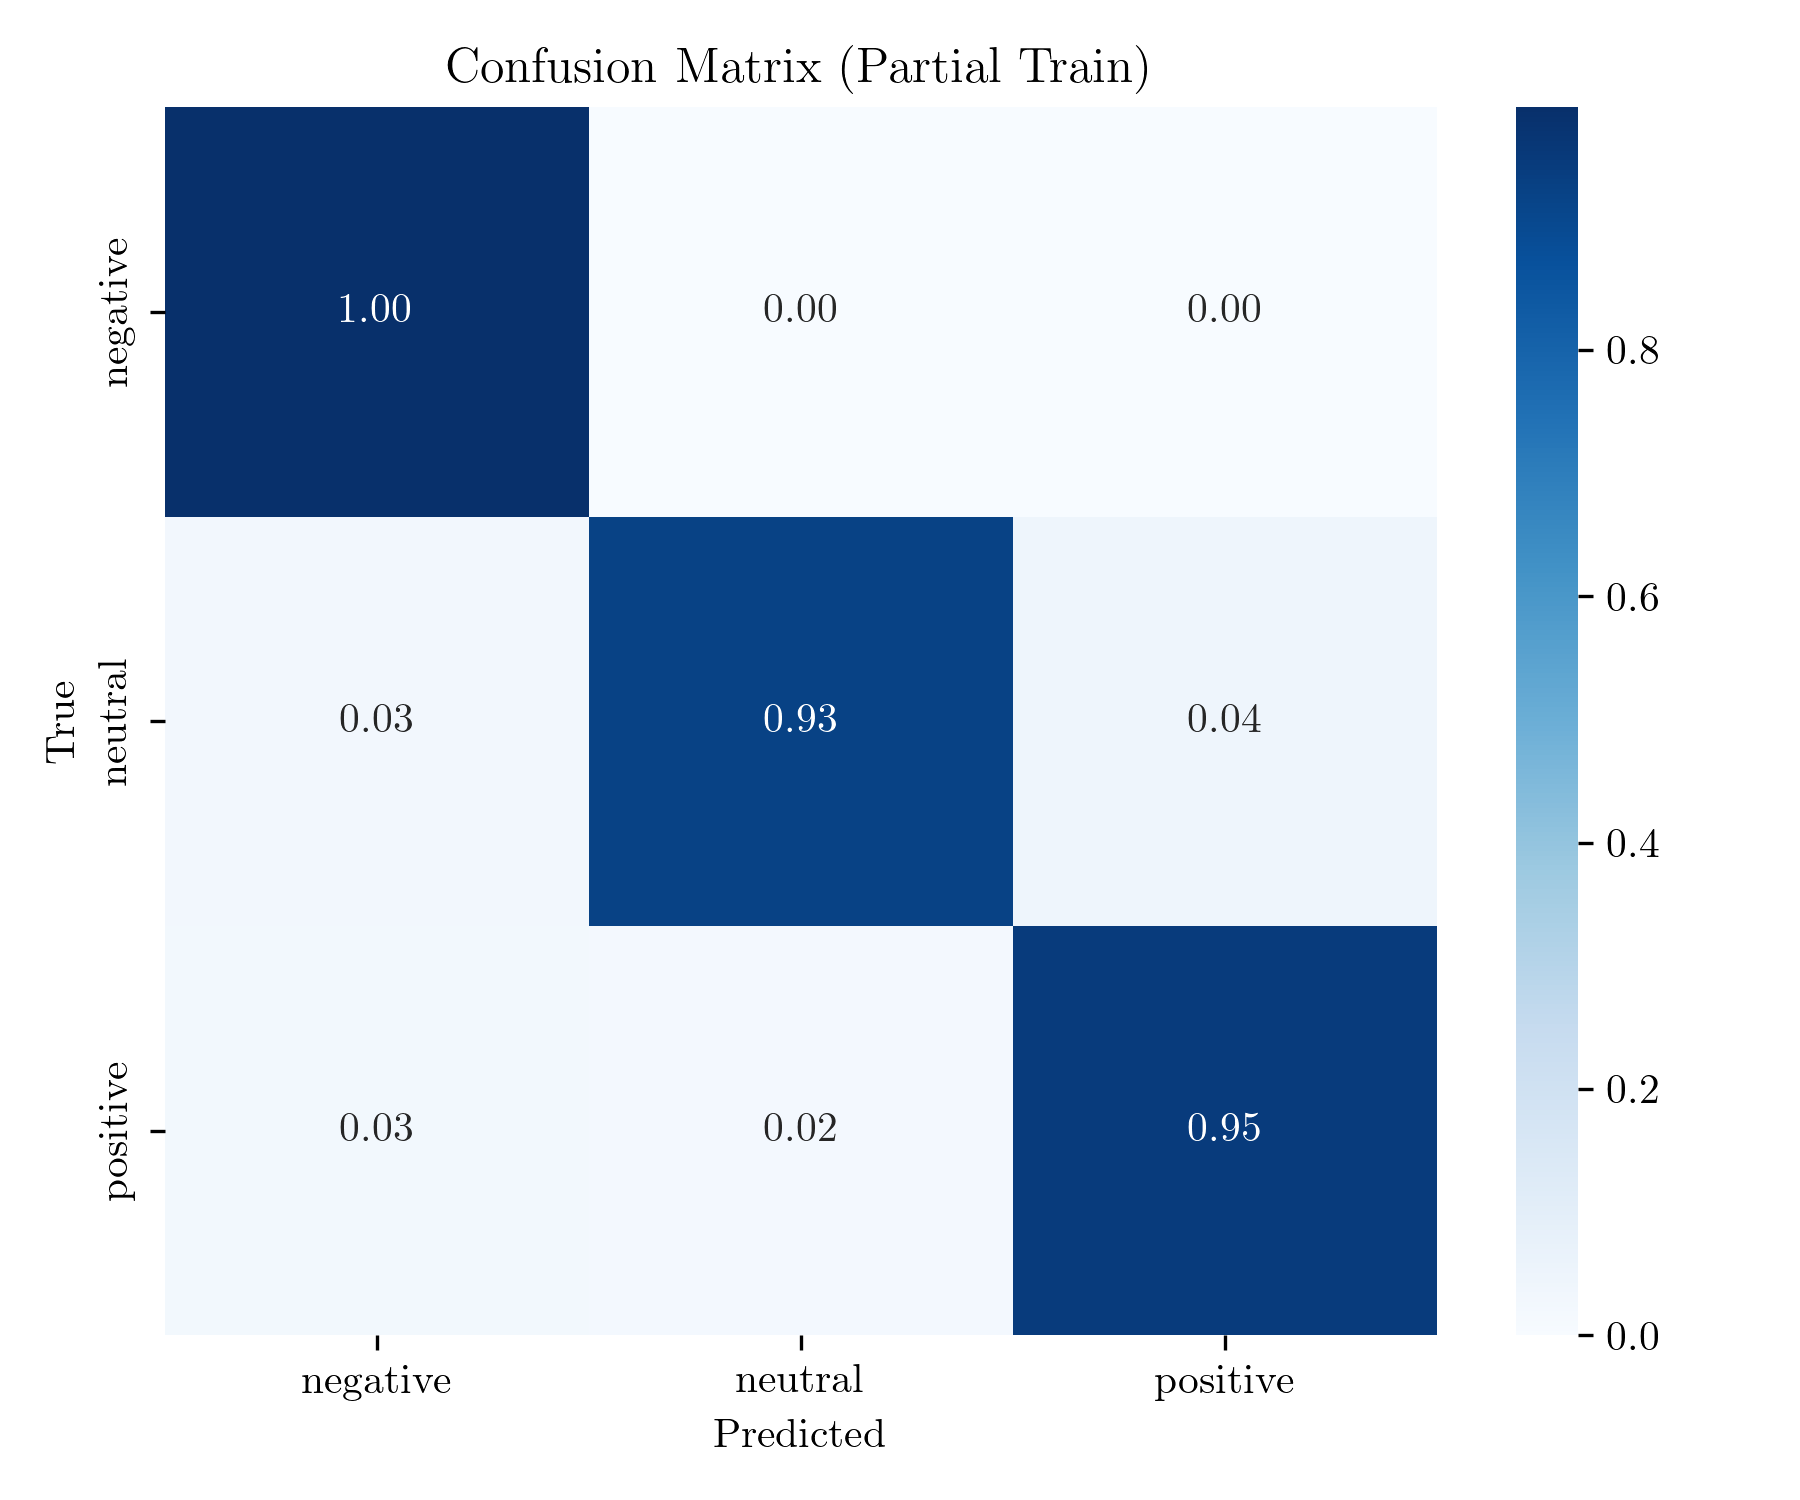
\includegraphics[width=1\linewidth]{assets/weighted_bert_confusion_matrix_Partial Train.png}
    \caption{Normalized confusion matrix for W-BERT model on the partial training set.}
    \label{fig:weighted_bert_confusion_matrix_Partial}
\end{figure}

\begin{table}[H]
\centering
\caption{Classification report for W-BERT on the partial training set.}
\label{cr_weightbert_train}
\begin{tabular}{lcccccc}
\toprule
\textbf{Class} & \textbf{Precision} & \textbf{Recall} & \textbf{F1-Score} & \textbf{Support} \\
\midrule
Negative & 0.83 & 1.00 & 0.91 & 336 \\
Neutral & 0.99 & 0.93 & 0.96 & 1717 \\
Positive & 0.90 & 0.85 & 0.93 & 709 \\
\midrule
\textbf{Accuracy} &  &  & 0.94 & 2762 \\
\textbf{Macro avg} & 0.91 & 0.96 & 0.93 & 2762 \\
\textbf{Weighted avg} & 0.95 & 0.94 & 0.94 & 2762 \\
\bottomrule
\end{tabular}
\end{table}

The confusion matrix on the test set (Fig. \ref{fig:weighted_bert_confusion_matrix_Test}) and the classification report (Table \ref{cr_wbert_test}) show a slight decrease in performance metrics, but overall well fit to the data. From the confusion matrix there doesn't seem a considerable change in identifying the classes, nor a straightforward interpretation of any two classes.

\begin{figure}[H]
    \centering
    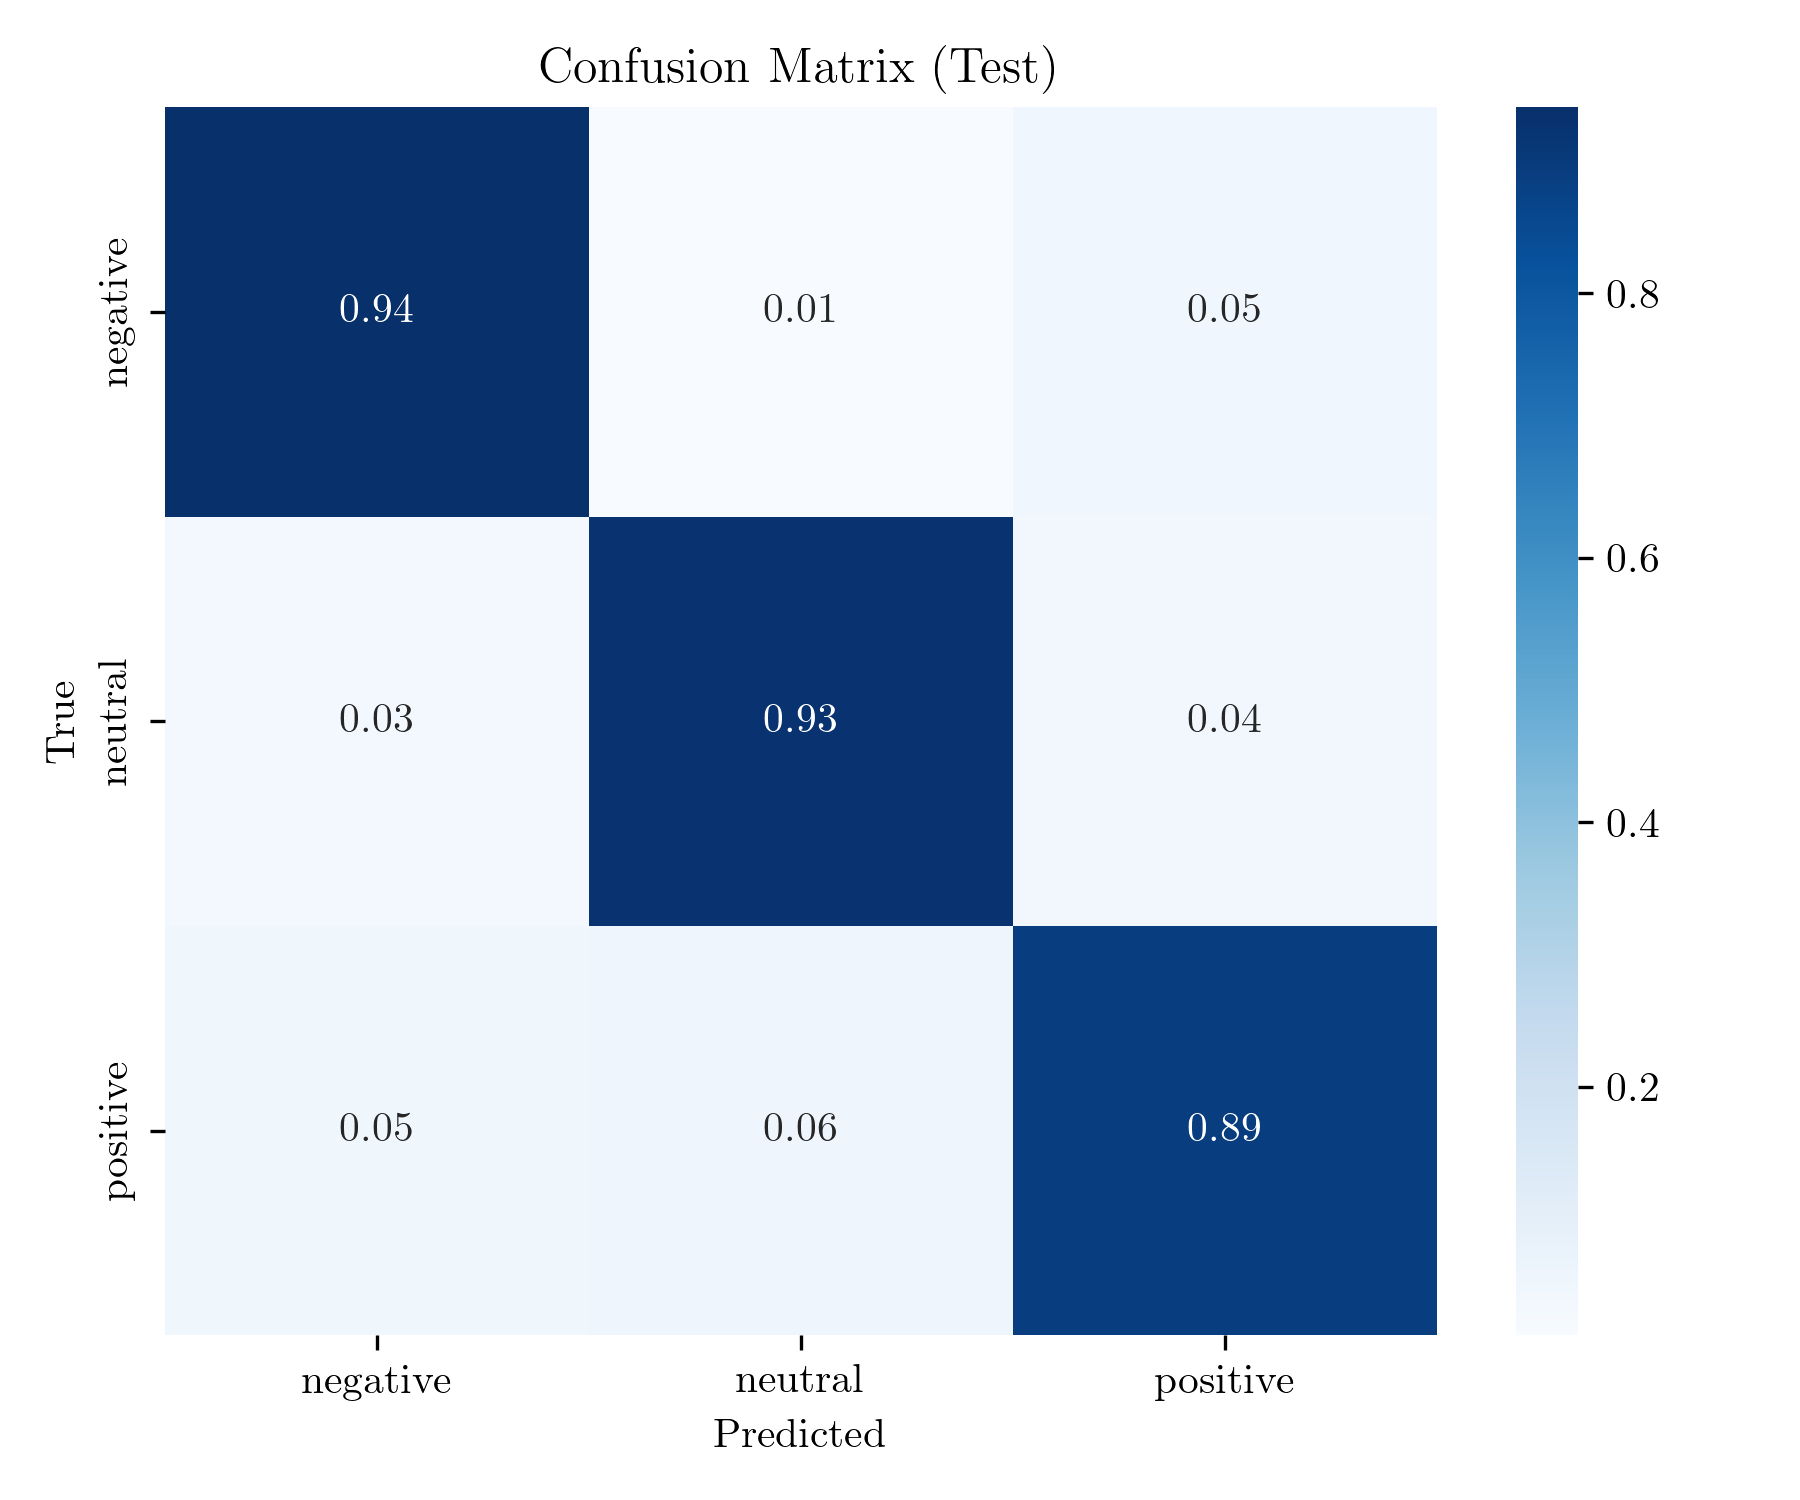
\includegraphics[width=1\linewidth]{assets/weighted_bert_confusion_matrix_Test.png}
    \caption{Normalized confusion matrix for W-BERT model on test data.}
    \label{fig:weighted_bert_confusion_matrix_Test}
\end{figure}

\begin{table}[H]
\centering
\caption{Classification report for W-BERT on test data.}
\label{cr_wbert_test}
\begin{tabular}{lcccccc}
\toprule
\textbf{Class} & \textbf{Precision} & \textbf{Recall} & \textbf{F1-Score} & \textbf{Support} \\
\midrule
Negative & 0.78 & 0.94 & 0.85 & 84 \\
Neutral & 0.97 & 0.93 & 0.95 & 429 \\
Positive & 0.88 & 0.89 & 0.89 & 178 \\
\midrule
\textbf{Accuracy} &  &  & 0.92 & 691 \\
\textbf{Macro avg} & 0.88 & 0.92 & 0.90 & 691 \\
\textbf{Weighted avg} & 0.93 & 0.92 & 0.92 & 691 \\
\bottomrule
\end{tabular}
\end{table}

These results may be further improved by implementing more precise methods for determining the raw agreement weight between annotators, whether through expert-driven refinement or fine-tuning. Additional gains could also be obtained by revisiting the weighting strategy applied during the training procedure.

\section{Discussion}

The metrics of the three BERT model variants are displayed in Fig. \ref{fig:results_radarchart}. At first glance, the B-BERT model slightly outperforms the other two, but only by narrow margins. Given that the test set likely shares significant similarities with the training set, and based on its detailed performance analysis, it is reasonable to conclude that the base model is overfitted and primarily suited to this specific setup. More importantly, the models designed for better generalization, DA-BERT and W-BERT, still perform well in this constrained scenario, with performance metrics closely matching those of the base model.

\begin{figure}[H]
    \centering
    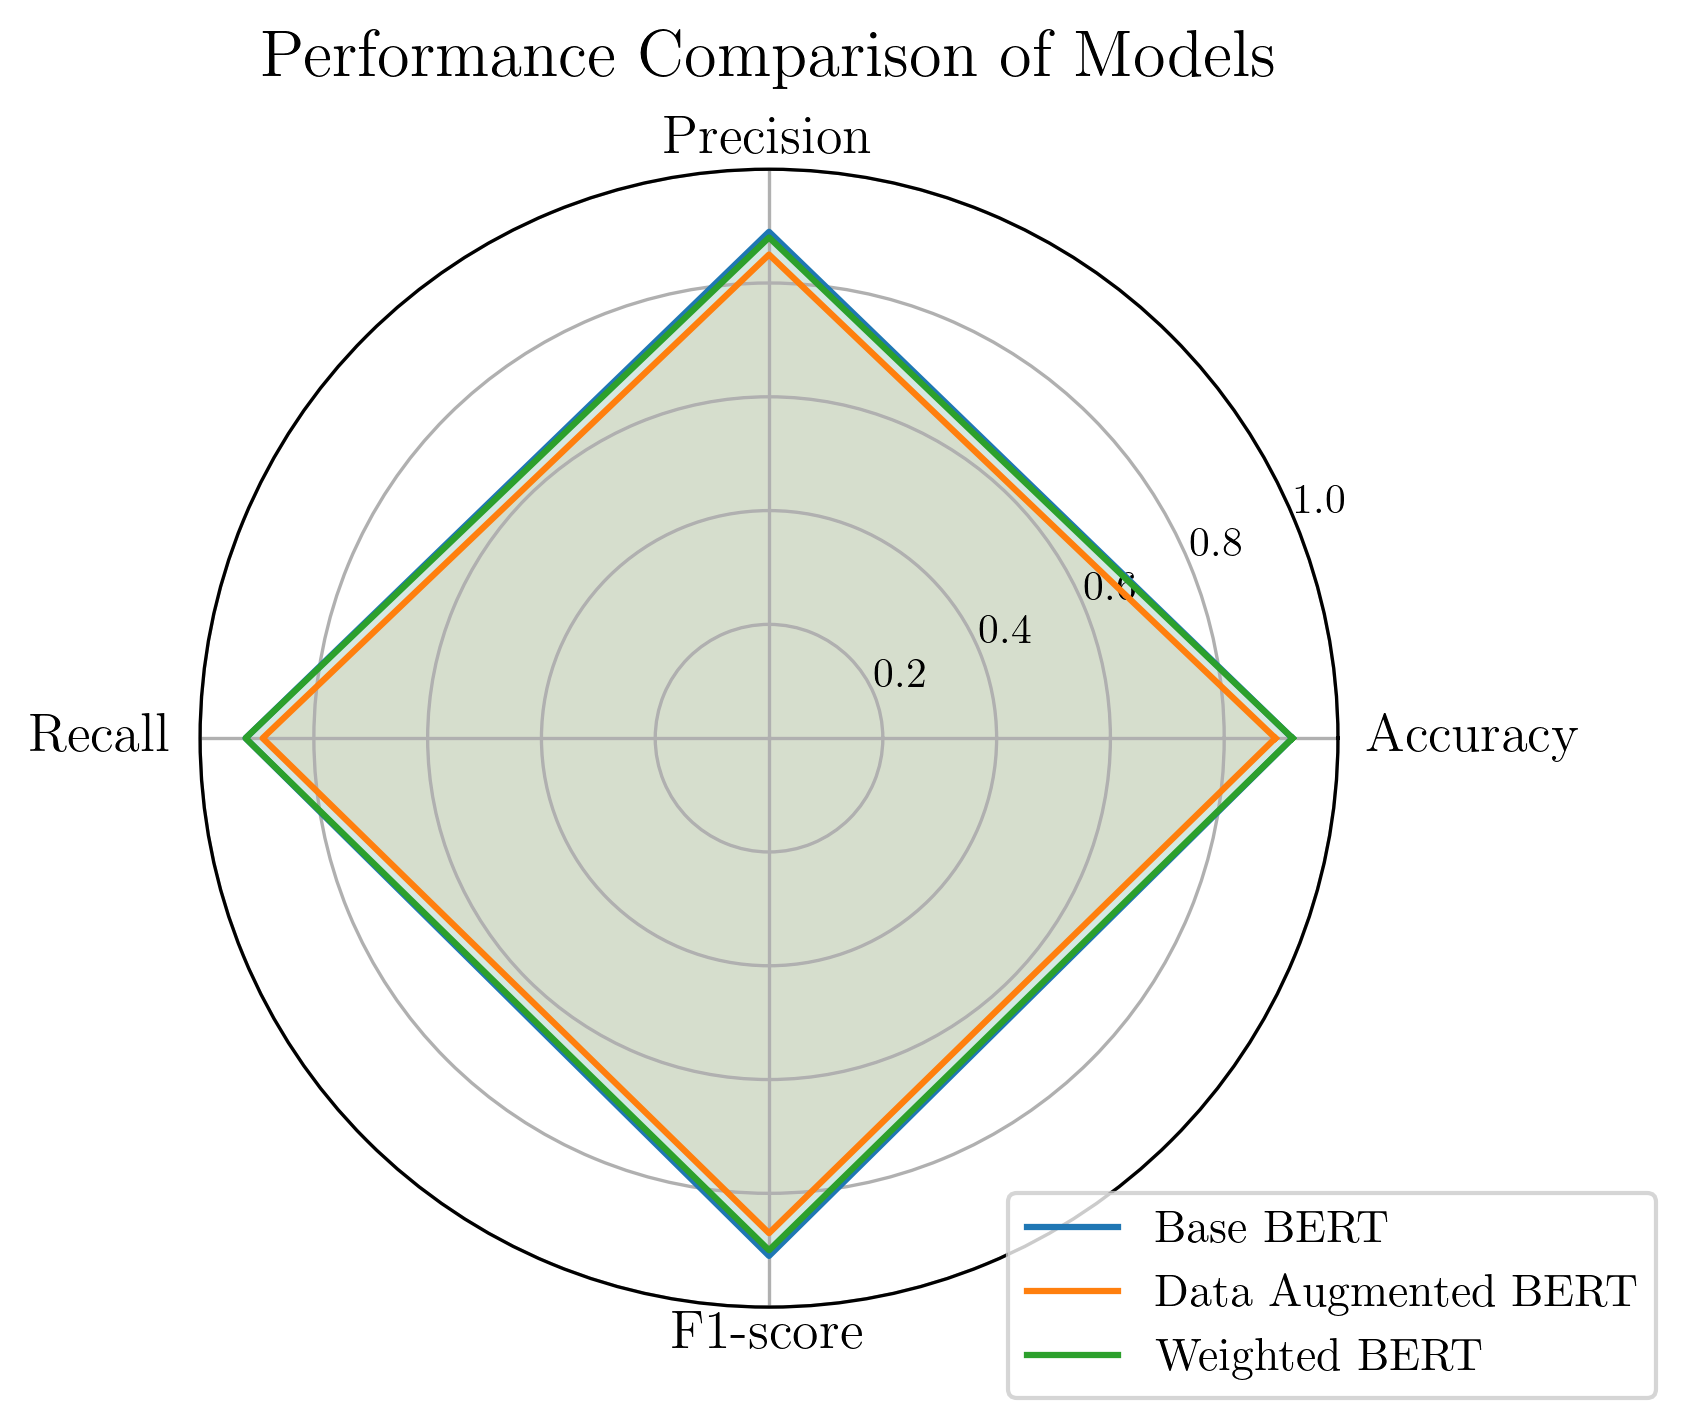
\includegraphics[width=1\linewidth]{assets/results_radarchart.png}
    \caption{Radar chart of the macro performance metrics of the BERT models.}
    \label{fig:results_radarchart}
\end{figure}

The models performed well in comparison with the literature, as shown in Table \ref{results_table}. While the results vary depending on the agreement level of the test set, the trained models consistently fall within the benchmark range reported in previous studies.

\begin{table}[H]
\centering
\caption{Performance comparison on the test set between the trained models and literature baselines.}
\label{results_table}
\begin{tabular}{lccc}
\toprule
\textbf{Model} & \textbf{Accuracy} & \textbf{F1 (macro)} & \textbf{Agreement Level} \\
\midrule
B-BERT & 0.92 & 0.91 & 75\% \\
DA-BERT & 0.89 & 0.87 & 75\% \\
W-BERT & 0.92 & 0.90 & 75\% \\
\midrule
Sun \textit{et al.} (2025) & - & 0.98 & 100\% \\
Sun \textit{et al.} (2025) & - & 0.87 & 50\% \\
Atsiwo (2024) & 0.89 & 0.88 & 50\% \\
Choe (2023) & 0.86 & 0.84 & not reported \\
Araci (2019) & 0.87 & 0.95 & 100\% \\
Araci (2019) & 0.86 & 0.84 & 50\% \\
Malo (2014) & 0.85 & 0.78 & 75\% \\
\bottomrule
\end{tabular}
\end{table}

\section{Conclusion}

This work explored different machine learning and deep learning models to perform sentiment classification in financial statements. The approach was defined to assess different models, in order to further explore the best, considering literature's best practices. Among the tested models, BERT performed much better than fastText and LSTM, and was further developed by employing a data augmentation pipeline, and, separately, a weighted approach based on the agreement level. Both cases performed close to the initial model, but, due to improved generalization, showed slightly poorer performance metrics.

For future work, both strategies could be implemented simultaneously, with models tested on different datasets to minimize the impact of performance metrics being influenced by potential overfitting to the dataset. Additionally, the weighted approach requires further investigation, ideally through expert-informed methods, to reach a stage where the model can infer the level of confidence in its predictions based on sentence structure, wording, and other linguistic patterns.

\section*{Work Load}

Both authors contributed equally to the project.

\bibliographystyle{IEEEtran}
\bibliography{references}

\end{document}